\documentclass[11pt, a4paper]{article}

% ----- Packages -----
\usepackage[utf8]{inputenc}
\usepackage{amsmath, amssymb, amsthm, mathtools}
\usepackage{geometry}
\geometry{top=1in, bottom=1in, left=1in, right=1in}
\usepackage{float}
\usepackage{tikz}
\usepackage{xcolor}
\usepackage{booktabs}
\usepackage{siunitx}
\usepackage{graphicx}
\usepackage{fancyhdr}
\usepackage{lastpage}
\usepackage[colorlinks=true, linkcolor=black, citecolor=black, urlcolor=black]{hyperref}
\usepackage[capitalise, noabbrev]{cleveref}
\usetikzlibrary{arrows.meta, positioning, patterns, calc}
\usepackage{pgfplots}
\pgfplotsset{compat=1.18}
\usepackage{listings}
\lstset{
    basicstyle=\ttfamily\scriptsize,
    breaklines=true,
    frame=single,
    numbers=left,
    numberstyle=\tiny\color{gray},
    keywordstyle=\color{blue!80!black}\bfseries,
    commentstyle=\color{green!50!black}\itshape,
    stringstyle=\color{red!70!black},
    showstringspaces=false,
    tabsize=4,
    extendedchars=true,
    inputencoding=utf8,
    literate={₂}{{$_2$}}1 {₃}{{$_3$}}1 {₁}{{$_1$}}1
             {σ}{{$\sigma$}}1 {ε}{{$\varepsilon$}}1
             {Σ}{{$\Sigma$}}1 {α}{{$\alpha$}}1
             {ζ}{{$\zeta$}}1 {η}{{$\eta$}}1
             {ξ}{{$\xi$}}1 {φ}{{$\phi$}}1
             {Ω}{{$\Omega$}}1 {Γ}{{$\Gamma$}}1
             {∈}{{$\in$}}1 {≤}{{$\leq$}}1 {≥}{{$\geq$}}1 {≠}{{$\neq$}}1
}

% ----- Fancy Headers/Footers -----
\pagestyle{fancy}
\fancyhf{}
\fancyhead[L]{\small CE 512 --- Finite Element Method}
\fancyhead[R]{\small Homework 3}
\fancyfoot[C]{\small Page \thepage\ of \pageref{LastPage}}
\renewcommand{\headrulewidth}{0.4pt}
\renewcommand{\footrulewidth}{0.4pt}

% ----- TikZ Styles -----
\tikzset{
    feNode/.style={circle, draw=black, fill=white, thick, inner sep=0pt, minimum size=1.8mm},
    dimLine/.style={|<->|, >=Latex, thick}
}

\begin{document}

% ----- Title Page -----
\begin{titlepage}
\thispagestyle{empty}
\begin{center}
    \vspace*{1cm}
    
\includegraphics[width=0.45\textwidth]{../HW1/iyte_logo eng.pdf}\\[1.5cm]
    {\LARGE \textbf{Homework 3 --- Solutions}}\\[0.8cm]
    {\Large \textbf{CE 512 Finite Element Method}}\\[0.4cm]
    {\Large 2026 Spring}\\[2.5cm]
    {\large \textbf{Muhammet Ya\u{g}c\i o\u{g}lu}}\\[0.3cm]
    {\large Student No: 290204042}\\[2cm]
    {\large March 16, 2026}\\[1.5cm]
    {\normalsize GitHub: \url{https://github.com/adzetto/ce512-fem-lab}}
    \vfill
    {\normalsize \textit{\.{I}zmir Institute of Technology}\\Department of Civil Engineering}
\end{center}
\end{titlepage}

% ----- TOC -----
\tableofcontents
\newpage

% ======================================================================
\section{Problem Statement}\label{sec:problem}
% ======================================================================

A uniform elastic bar of length $L$, cross-sectional area $A$, and Young's modulus $E$ is fixed at the left end ($x=0$) and free at the right end ($x=L$).  Two concentrated loads, each of magnitude $P$, act in the positive $x$-direction: one at the mid-length $x=L/2$ and one at the right end $x=L$ (\cref{fig:problem}).

\begin{figure}[H]
\centering
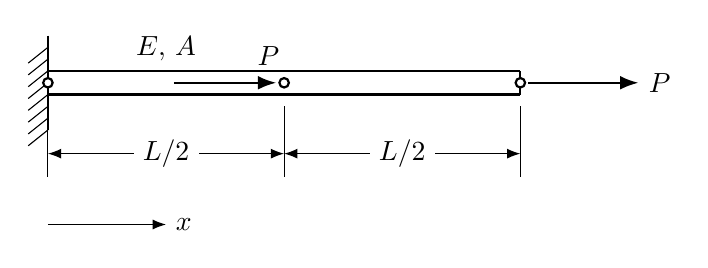
\begin{tikzpicture}[>=Latex, font=\sffamily]
    % 1. Fixed Support (Left Wall)
    \draw[thick] (0, 0.6) -- (0, -0.6);
    \foreach \y in {-0.6, -0.45, ..., 0.6} {
        \draw (0,\y) -- (-0.25,\y-0.2);
    }
    % 2. 1-D Bar Element (Hollow Profile)
    \draw[thick] (0, 0.15) -- (6, 0.15);
    \draw[thick] (0, -0.15) -- (6, -0.15);
    \draw[thick] (6, 0.15) -- (6, -0.15);
    % Material/Section Properties
    \node[above] at (1.5, 0.15) {$E,\,A$};
    % 3. Applied Loads (Vectors)
    \draw[thick, ->] (1.6, 0) -- (2.9, 0);
    \node[above] at (2.8, 0.1) {$P$};
    \draw[thick, ->] (6.1, 0) -- (7.5, 0) node[right] {$P$};
    % 4. Finite Element Nodes
    \filldraw[fill=white, draw=black, thick] (0,0) circle (0.06);
    \filldraw[fill=white, draw=black, thick] (3,0) circle (0.06);
    \filldraw[fill=white, draw=black, thick] (6,0) circle (0.06);
    % 5. Dimensions
    \draw (0, -0.3) -- (0, -1.2);
    \draw (3, -0.3) -- (3, -1.2);
    \draw (6, -0.3) -- (6, -1.2);
    \draw[<->] (0, -0.9) -- (3, -0.9) node[midway, fill=white] {$L/2$};
    \draw[<->] (3, -0.9) -- (6, -0.9) node[midway, fill=white] {$L/2$};
    % Coordinate axis
    \draw[->] (0, -1.8) -- (1.5, -1.8) node[right] {$x$};
\end{tikzpicture}
\caption{1-D bar element: fixed at left end, loads $P$ at $x=L/2$ and $x=L$.}
\label{fig:problem}
\end{figure}

\noindent\textbf{Required:}
\begin{enumerate}
    \item[(a)] Find $a_2$ for $u(x) = a_2 x^2$.
    \item[(b)] Find $a_2, a_3$ for $u(x) = a_2 x^2 + a_3 x^3$.
    \item[(c)] Plot the displacement fields from (a) and (b) on a single graph.
    \item[(d)] Plot the stress variation for (a) and (b) on a single graph.
\end{enumerate}

% ======================================================================
\section{Potential Energy Functional}\label{sec:functional}
% ======================================================================

Let $\varepsilon_x=u_{,x}$, $\sigma_x=E\varepsilon_x$.  Total potential energy:
\begin{equation}\label{eq:pi}
\Pi_p = U + \Omega = \frac{EA}{2}\int_0^L u_{,x}^2\,dx - P\,u\!\left(\tfrac{L}{2}\right) - P\,u(L)
\end{equation}

Essential BC: $u(0)=0$.  Both trial functions satisfy this automatically.

Let $u(x)=\sum_j a_j\,\phi_j(x)$ with $\phi_j(x)=x^j$.  Stationarity $\partial\Pi_p/\partial a_i=0$ gives
\begin{equation}\label{eq:rr_general}
[\mathbf{K}]\{\mathbf{a}\} = \{\mathbf{F}\}
\end{equation}
\begin{equation}\label{eq:KF_entries}
K_{ij} = EA\int_0^L \phi_i'(x)\,\phi_j'(x)\,dx,\qquad
F_i = P\,\phi_i\!\left(\tfrac{L}{2}\right) + P\,\phi_i(L)
\end{equation}

% ======================================================================
\section{Part (a): One-Term Approximation, \texorpdfstring{$u(x) = a_2 x^2$}{u(x)=a2 x2}}\label{sec:parta}
% ======================================================================

\subsection{Derivation}

Let $\phi_2(x)=x^2$, $\phi_2'(x)=2x$, so $u(x)=a_2\,x^2$, $u_{,x}=2a_2\,x$.

\paragraph{Stiffness coefficient $K_{22}$.}
\begin{align}
K_{22} &= EA\int_0^L \phi_2'(x)\;\phi_2'(x)\,dx
       = EA\int_0^L (2x)(2x)\,dx \notag\\[6pt]
       &= 4\,EA\int_0^L x^2\,dx
       = 4\,EA\left[\frac{x^3}{3}\right]_{\!0}^{\!L} \notag\\[6pt]
       &= 4\,EA\cdot\frac{L^3}{3}
       = \frac{4\,EAL^3}{3} \label{eq:K22_a}
\end{align}

\paragraph{Force coefficient $F_2$.}
\begin{align}
F_2 &= P\,\phi_2\!\left(\frac{L}{2}\right) + P\,\phi_2(L)
     = P\!\left(\frac{L}{2}\right)^{\!2} + P\,L^2 \notag\\[6pt]
    &= \frac{PL^2}{4} + PL^2
     = \frac{PL^2}{4} + \frac{4PL^2}{4}
     = \frac{5PL^2}{4} \label{eq:F2_a}
\end{align}

\paragraph{Strain energy (via $K_{22}$).}
\begin{equation}
U = \tfrac{1}{2}\,a_2\,K_{22}\,a_2 = \tfrac{1}{2}\cdot\frac{4EAL^3}{3}\,a_2^2 = \frac{2EAL^3}{3}\,a_2^2
\end{equation}

\paragraph{Total potential energy.}
\begin{equation}\label{eq:pi_a}
\Pi_p = U + \Omega = \frac{2EAL^3}{3}\,a_2^2 - \frac{5PL^2}{4}\,a_2
\end{equation}

\paragraph{Stationarity.}
$\partial\Pi_p/\partial a_2=0$:
\begin{align*}
\frac{\partial\Pi_p}{\partial a_2}
&= \frac{4EAL^3}{3}\,a_2 - \frac{5PL^2}{4} = 0
\qquad\Longrightarrow\qquad K_{22}\,a_2 = F_2
\end{align*}

\paragraph{Solving for $a_2$.}
\begin{align*}
a_2 &= \frac{F_2}{K_{22}}
     = \frac{\;\dfrac{5PL^2}{4}\;}{\;\dfrac{4EAL^3}{3}\;}
     = \frac{5PL^2}{4}\cdot\frac{3}{4EAL^3} \\[8pt]
    &= \frac{5\cdot 3\;P\,L^2}{4\cdot 4\;EA\,L^3}
     = \frac{15\,P}{16\,EA\,L}
\end{align*}

\begin{equation}\label{eq:a2_parta}
\boxed{a_2 = \frac{15\,P}{16\,EAL}}
\end{equation}

\subsection{Displacement and Stress Fields}

\begin{equation}\label{eq:u_a}
\boxed{u_a(x) = \frac{15P}{16\,EAL}\,x^2}
\end{equation}

\begin{equation}\label{eq:sigma_a}
\sigma_a(x) = E\,u_{a,x} = E\cdot\frac{15P\cdot 2x}{16\,EAL} = \frac{15\,P\,x}{8\,A\,L}
\end{equation}

\noindent Key values:
\[
u_a\!\left(\frac{L}{2}\right) = \frac{15PL}{64\,EA},\qquad
u_a(L) = \frac{15PL}{16\,EA},\qquad
\sigma_a(0) = 0,\qquad
\sigma_a(L) = \frac{15P}{8A}.
\]

% ======================================================================
\section{Part (b): Two-Term Approximation, \texorpdfstring{$u(x) = a_2 x^2 + a_3 x^3$}{u(x)=a2 x2+a3 x3}}\label{sec:partb}
% ======================================================================

\subsection{Derivation}

Let $\phi_2=x^2$, $\phi_3=x^3$, so $\phi_2'=2x$, $\phi_3'=3x^2$, $u=a_2 x^2+a_3 x^3$, $u_{,x}=2a_2 x+3a_3 x^2$.

\paragraph{Stiffness coefficients $K_{ij}$.}

\noindent$K_{22}$:
\begin{align*}
K_{22} &= EA\int_0^L \phi_2'\,\phi_2'\,dx
       = EA\int_0^L (2x)(2x)\,dx
       = 4\,EA\int_0^L x^2\,dx \\[4pt]
       &= 4\,EA\cdot\frac{L^3}{3}
       = \frac{4\,EAL^3}{3}
\end{align*}

\noindent$K_{23}=K_{32}$ (symmetry):
\begin{align*}
K_{23} &= EA\int_0^L \phi_2'\,\phi_3'\,dx
       = EA\int_0^L (2x)(3x^2)\,dx
       = 6\,EA\int_0^L x^3\,dx \\[4pt]
       &= 6\,EA\cdot\frac{L^4}{4}
       = \frac{6\,EAL^4}{4}
       = \frac{3\,EAL^4}{2}
\end{align*}

\noindent$K_{33}$:
\begin{align*}
K_{33} &= EA\int_0^L \phi_3'\,\phi_3'\,dx
       = EA\int_0^L (3x^2)(3x^2)\,dx
       = 9\,EA\int_0^L x^4\,dx \\[4pt]
       &= 9\,EA\cdot\frac{L^5}{5}
       = \frac{9\,EAL^5}{5}
\end{align*}

\paragraph{Force coefficients $F_i$.}

\noindent$F_2$:
\begin{align*}
F_2 &= P\,\phi_2\!\left(\frac{L}{2}\right)+P\,\phi_2(L)
     = P\!\left(\frac{L}{2}\right)^{\!2}+P\,L^2
     = \frac{PL^2}{4}+PL^2
     = \frac{5PL^2}{4}
\end{align*}

\noindent$F_3$:
\begin{align*}
F_3 &= P\,\phi_3\!\left(\frac{L}{2}\right)+P\,\phi_3(L)
     = P\!\left(\frac{L}{2}\right)^{\!3}+P\,L^3
     = \frac{PL^3}{8}+PL^3
     = \frac{PL^3+8PL^3}{8}
     = \frac{9PL^3}{8}
\end{align*}

\paragraph{Strain energy (check).}
\begin{align*}
u_{,x}^2 &= (2a_2 x+3a_3 x^2)^2
           = 4a_2^2\,x^2+12\,a_2 a_3\,x^3+9a_3^2\,x^4 \\[6pt]
U &= \frac{EA}{2}\int_0^L\!\big(4a_2^2\,x^2+12\,a_2 a_3\,x^3+9a_3^2\,x^4\big)\,dx \\[4pt]
  &= \frac{EA}{2}\left[4a_2^2\cdot\frac{L^3}{3}+12\,a_2 a_3\cdot\frac{L^4}{4}+9a_3^2\cdot\frac{L^5}{5}\right] \\[4pt]
  &= EA\left[\frac{2a_2^2 L^3}{3}+\frac{3\,a_2 a_3 L^4}{2}+\frac{9a_3^2 L^5}{10}\right]
   = \frac{1}{2}\,a_i\,K_{ij}\,a_j \;\;\checkmark
\end{align*}

\paragraph{Potential of external forces.}
\begin{align*}
u\!\left(\frac{L}{2}\right) &= a_2\!\left(\frac{L}{2}\right)^{\!2}+a_3\!\left(\frac{L}{2}\right)^{\!3}
                              = \frac{a_2 L^2}{4}+\frac{a_3 L^3}{8} \\[6pt]
u(L) &= a_2 L^2+a_3 L^3 \\[6pt]
\Omega &= -P\,u\!\left(\frac{L}{2}\right)-P\,u(L) \\[2pt]
       &= -P\left[\frac{a_2 L^2}{4}+\frac{a_3 L^3}{8}+a_2 L^2+a_3 L^3\right] \\[2pt]
       &= -P\left[\left(\frac{1}{4}+1\right)a_2 L^2+\left(\frac{1}{8}+1\right)a_3 L^3\right]
        = -P\left[\frac{5a_2 L^2}{4}+\frac{9a_3 L^3}{8}\right]
\end{align*}

\paragraph{Total potential energy.}
\begin{equation}\label{eq:pi_b}
\Pi_p = EA\left[\frac{2L^3}{3}\,a_2^2+\frac{3L^4}{2}\,a_2 a_3+\frac{9L^5}{10}\,a_3^2\right]
       -P\left[\frac{5L^2}{4}\,a_2+\frac{9L^3}{8}\,a_3\right]
\end{equation}

\paragraph{Stationarity.}
$\partial\Pi_p/\partial a_i=0$:
\begin{align}
\frac{\partial\Pi_p}{\partial a_2}
&= EA\left[\frac{4L^3}{3}\,a_2+\frac{3L^4}{2}\,a_3\right]-\frac{5PL^2}{4}=0
\label{eq:stat1}\\[8pt]
\frac{\partial\Pi_p}{\partial a_3}
&= EA\left[\frac{3L^4}{2}\,a_2+\frac{9L^5}{5}\,a_3\right]-\frac{9PL^3}{8}=0
\label{eq:stat2}
\end{align}

In matrix form $[\mathbf{K}]\{\mathbf{a}\}=\{\mathbf{F}\}$:
\begin{equation}\label{eq:system_b}
EA\begin{bmatrix} \dfrac{4L^3}{3} & \dfrac{3L^4}{2} \\[12pt] \dfrac{3L^4}{2} & \dfrac{9L^5}{5} \end{bmatrix}\begin{Bmatrix} a_2 \\[10pt] a_3 \end{Bmatrix} = P\begin{Bmatrix} \dfrac{5L^2}{4} \\[10pt] \dfrac{9L^3}{8} \end{Bmatrix}
\end{equation}

\subsection{Solution of the \texorpdfstring{$2\times 2$}{2x2} System}

\paragraph{Determinant.}
$\det[\mathbf{K}]=K_{22}K_{33}-K_{23}^2$:
\begin{align*}
K_{22}\,K_{33} &= \frac{4EAL^3}{3}\cdot\frac{9EAL^5}{5}
                = \frac{36\,(EA)^2 L^8}{15}
                = \frac{12\,(EA)^2 L^8}{5} \\[6pt]
K_{23}^2 &= \left(\frac{3EAL^4}{2}\right)^{\!2}
           = \frac{9\,(EA)^2 L^8}{4} \\[6pt]
\det[\mathbf{K}] &= \frac{12\,(EA)^2 L^8}{5}-\frac{9\,(EA)^2 L^8}{4}
                   = (EA)^2 L^8\!\left(\frac{12}{5}-\frac{9}{4}\right) \\[4pt]
                  &= (EA)^2 L^8\cdot\frac{48-45}{20}
                   = \frac{3\,(EA)^2 L^8}{20}
\end{align*}

\paragraph{Inverse.}
$[\mathbf{K}]^{-1}=\frac{1}{\det[\mathbf{K}]}\begin{bsmallmatrix}K_{33}&-K_{23}\\-K_{32}&K_{22}\end{bsmallmatrix}$:
\begin{align*}
[\mathbf{K}]^{-1}
&= \frac{20}{3\,(EA)^2 L^8}\begin{bmatrix} \dfrac{9EAL^5}{5} & -\dfrac{3EAL^4}{2} \\[10pt] -\dfrac{3EAL^4}{2} & \dfrac{4EAL^3}{3} \end{bmatrix} \\[10pt]
&= \frac{1}{EA}\begin{bmatrix} \dfrac{20\cdot 9}{3\cdot 5\,L^3} & \dfrac{-20\cdot 3}{3\cdot 2\,L^4} \\[10pt] \dfrac{-20\cdot 3}{3\cdot 2\,L^4} & \dfrac{20\cdot 4}{3\cdot 3\,L^5} \end{bmatrix}
= \frac{1}{EA}\begin{bmatrix} \dfrac{12}{L^3} & -\dfrac{10}{L^4} \\[10pt] -\dfrac{10}{L^4} & \dfrac{80}{9L^5} \end{bmatrix}
\end{align*}

\paragraph{Computing $a_2$.}
\begin{align*}
a_2 &= (K^{-1})_{22}\,F_2+(K^{-1})_{23}\,F_3 \\[4pt]
    &= \frac{1}{EA}\!\left[\frac{12}{L^3}\cdot\frac{5PL^2}{4}
      -\frac{10}{L^4}\cdot\frac{9PL^3}{8}\right] \\[6pt]
    &= \frac{P}{EA}\!\left[\frac{60}{4L}-\frac{90}{8L}\right]
     = \frac{P}{EA}\!\left[\frac{15}{L}-\frac{45}{4L}\right] \\[6pt]
    &= \frac{P}{EA}\cdot\frac{60-45}{4L}
     = \frac{15\,P}{4\,EA\,L}
\end{align*}

\paragraph{Computing $a_3$.}
\begin{align*}
a_3 &= (K^{-1})_{32}\,F_2+(K^{-1})_{33}\,F_3 \\[4pt]
    &= \frac{1}{EA}\!\left[-\frac{10}{L^4}\cdot\frac{5PL^2}{4}
      +\frac{80}{9L^5}\cdot\frac{9PL^3}{8}\right] \\[6pt]
    &= \frac{P}{EA}\!\left[-\frac{50}{4L^2}+\frac{720}{72\,L^2}\right]
     = \frac{P}{EA}\!\left[-\frac{50}{4L^2}+\frac{10}{L^2}\right] \\[6pt]
    &= \frac{P}{EA}\cdot\frac{-50+40}{4L^2}
     = -\frac{10\,P}{4\,EA\,L^2}
     = -\frac{5\,P}{2\,EA\,L^2}
\end{align*}

\begin{equation}\label{eq:a_partb}
\boxed{a_2 = \frac{15\,P}{4\,EAL},\qquad a_3 = -\frac{5\,P}{2\,EAL^2}}
\end{equation}

\subsection{Verification}

Substituting back into \cref{eq:stat1}:
\[
EA\left[\frac{4L^3}{3}\cdot\frac{15P}{4EAL} + \frac{3L^4}{2}\cdot\frac{-5P}{2EAL^2}\right] = 5PL^2 - \frac{15PL^2}{4} = \frac{5PL^2}{4}\;\checkmark
\]

Substituting back into \cref{eq:stat2}:
\[
EA\left[\frac{3L^4}{2}\cdot\frac{15P}{4EAL} + \frac{9L^5}{5}\cdot\frac{-5P}{2EAL^2}\right] = \frac{45PL^3}{8} - \frac{9PL^3}{2} = \frac{9PL^3}{8}\;\checkmark
\]

\subsection{Displacement and Stress Fields}

\begin{equation}\label{eq:u_b}
\boxed{u_b(x) = \frac{15\,P}{4\,EAL}\,x^2 - \frac{5\,P}{2\,EAL^2}\,x^3 = \frac{5\,P\,x^2}{4\,EAL}\!\left(3 - \frac{2x}{L}\right)}
\end{equation}

The stress:
\begin{align}
\sigma_b(x) &= E\,u_{b,x} = E\left(\frac{30\,P\,x}{4\,EAL} - \frac{15\,P\,x^2}{2\,EAL^2}\right) = \frac{15\,P\,x}{2\,A\,L}\!\left(1 - \frac{x}{L}\right) \label{eq:sigma_b}
\end{align}

\begin{equation}\label{eq:sigma_b_box}
\boxed{\sigma_b(x) = \frac{15\,P\,x\,(L - x)}{2\,A\,L^2}}
\end{equation}

\noindent Key values:
\[
u_b\!\left(\frac{L}{2}\right) = \frac{5PL}{8\,EA},\qquad
u_b(L) = \frac{5PL}{4\,EA},\qquad
\sigma_b(0) = 0,\qquad
\sigma_b\!\left(\frac{L}{2}\right) = \frac{15P}{8A},\qquad
\sigma_b(L) = 0.
\]

% ======================================================================
\section{Exact Solution}\label{sec:exact}
% ======================================================================

\paragraph{Internal force.}
Cut at $0<x<L/2$: $N(x)=2P$.  Cut at $L/2<x<L$: $N(x)=P$.
\[
N(x) = \begin{cases} 2P & 0 \le x < L/2 \\ P & L/2 < x \le L \end{cases}
\]

\paragraph{Displacement.}
$\varepsilon(x)=N(x)/(EA)$, integrate from $u(0)=0$.  For $0\le x\le L/2$:
\begin{align*}
u(x) &= \int_0^x \frac{N(\xi)}{EA}\,d\xi
      = \int_0^x \frac{2P}{EA}\,d\xi
      = \frac{2P}{EA}\,x
\end{align*}

At $x=L/2$:\quad $u(L/2)=\dfrac{2P}{EA}\cdot\dfrac{L}{2}=\dfrac{PL}{EA}$.

For $L/2\le x\le L$:
\begin{align*}
u(x) &= u\!\left(\frac{L}{2}\right)+\int_{L/2}^x \frac{N(\xi)}{EA}\,d\xi
      = \frac{PL}{EA}+\int_{L/2}^x \frac{P}{EA}\,d\xi \\[6pt]
     &= \frac{PL}{EA}+\frac{P}{EA}\!\left(x-\frac{L}{2}\right)
      = \frac{PL}{EA}+\frac{Px}{EA}-\frac{PL}{2EA} \\[6pt]
     &= \frac{P}{EA}\!\left(\frac{L}{2}+x\right)
\end{align*}

\begin{equation}\label{eq:u_exact}
\boxed{u_{\text{exact}}(x) = \begin{cases} \dfrac{2Px}{EA} & 0 \le x \le L/2 \\[10pt] \dfrac{P(L/2+x)}{EA} & L/2 \le x \le L \end{cases}}
\end{equation}

At $x=L$:\quad $u(L)=\dfrac{P}{EA}\!\left(\dfrac{L}{2}+L\right)=\dfrac{3PL}{2EA}$.

\paragraph{Exact stress.}
\begin{equation}\label{eq:sigma_exact}
\sigma_{\text{exact}}(x)=\frac{N(x)}{A}=\begin{cases} \dfrac{2P}{A} & 0 \le x < L/2 \\[8pt] \dfrac{P}{A} & L/2 < x \le L \end{cases}
\end{equation}

\paragraph{Key exact values.}
\[
u_{\text{exact}}\!\left(\frac{L}{2}\right)=\frac{PL}{EA},\qquad
u_{\text{exact}}(L)=\frac{3PL}{2\,EA},\qquad
\sigma_{\text{exact}}(0^+)=\frac{2P}{A},\qquad
\sigma_{\text{exact}}(L)=\frac{P}{A}.
\]

% ======================================================================
\section{Part (c): Displacement Plots}\label{sec:partc}
% ======================================================================

\cref{fig:displacement} compares the two Rayleigh-Ritz approximations and the exact displacement field.  All quantities are non-dimensionalised using $\bar{x} = x/L$ and $\bar{u} = u\cdot EA/(PL)$.

\begin{align}
\bar{u}_a(\bar{x}) &= \frac{15}{16}\,\bar{x}^2 \label{eq:ubar_a}\\[4pt]
\bar{u}_b(\bar{x}) &= \frac{15}{4}\,\bar{x}^2 - \frac{5}{2}\,\bar{x}^3 \label{eq:ubar_b}\\[4pt]
\bar{u}_{\text{exact}}(\bar{x}) &= \begin{cases} 2\bar{x} & 0\le\bar{x}\le 0.5 \\ 0.5 + \bar{x} & 0.5\le\bar{x}\le 1 \end{cases}\label{eq:ubar_exact}
\end{align}

\begin{figure}[H]
\centering
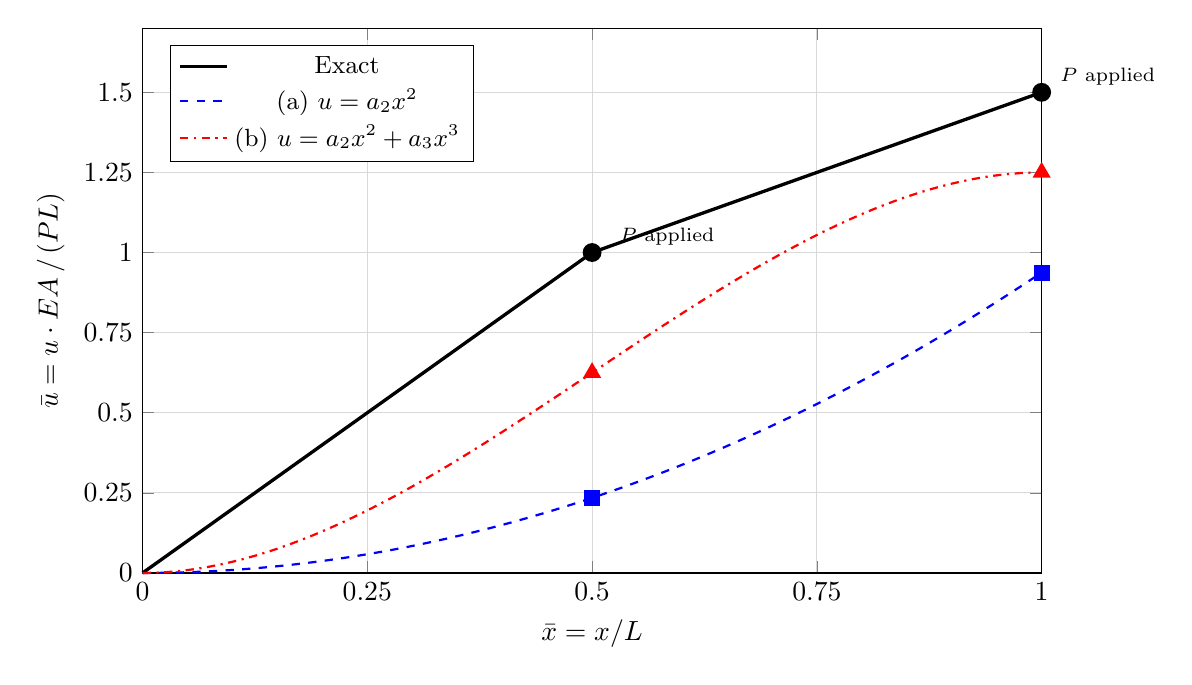
\begin{tikzpicture}
\begin{axis}[
    width=13cm, height=8.5cm,
    xlabel={$\bar{x} = x/L$},
    ylabel={$\bar{u} = u \cdot EA \,/\, (PL)$},
    xmin=0, xmax=1,
    ymin=0, ymax=1.7,
    xtick={0, 0.25, 0.5, 0.75, 1.0},
    ytick={0, 0.25, 0.5, 0.75, 1.0, 1.25, 1.5},
    grid=major,
    grid style={gray!30},
    legend style={at={(0.03,0.97)}, anchor=north west, font=\small},
    every axis plot/.append style={thick},
    clip=false
]

% Exact solution (piecewise linear)
\addplot[black, very thick, solid, domain=0:0.5, samples=2] {2*x};
\addplot[black, very thick, solid, domain=0.5:1, samples=2, forget plot] {0.5+x};
\addlegendentry{Exact}

% Part a) - one term
\addplot[blue, thick, dashed, domain=0:1, samples=80] {(15/16)*x^2};
\addlegendentry{(a) $u = a_2 x^2$}

% Part b) - two terms
\addplot[red, thick, dashdotted, domain=0:1, samples=80] {(15/4)*x^2 - (5/2)*x^3};
\addlegendentry{(b) $u = a_2 x^2 + a_3 x^3$}

% Mark load application points
\addplot[only marks, mark=*, mark size=3pt, black] coordinates {(0.5, 1.0) (1.0, 1.5)};
\addplot[only marks, mark=square*, mark size=2.5pt, blue] coordinates {(0.5, 0.234375) (1.0, 0.9375)};
\addplot[only marks, mark=triangle*, mark size=3pt, red] coordinates {(0.5, 0.625) (1.0, 1.25)};

% Annotations
\node[anchor=west, font=\scriptsize] at (axis cs:0.52, 1.05) {$P$ applied};
\node[anchor=west, font=\scriptsize] at (axis cs:1.01, 1.55) {$P$ applied};

\end{axis}
\end{tikzpicture}
\caption{Non-dimensional displacement fields: exact solution vs.\ one-term and two-term Rayleigh-Ritz approximations.}
\label{fig:displacement}
\end{figure}

\begin{table}[H]
\centering
\renewcommand{\arraystretch}{1.4}
\begin{tabular}{@{}c c c c c c@{}}
\toprule
$\bar{x}$ & $\bar{u}_{\text{exact}}$ & $\bar{u}_a$ & Error (a) & $\bar{u}_b$ & Error (b) \\
\midrule
$0$   & $0$     & $0$     & ---     & $0$     & ---     \\
$0.5$ & $1.000$ & $0.234$ & $76.6\%$ & $0.625$ & $37.5\%$ \\
$1.0$ & $1.500$ & $0.938$ & $37.5\%$ & $1.250$ & $16.7\%$ \\
\bottomrule
\end{tabular}
\caption{Displacement comparison at key locations.  Error $= 1 - \bar{u}_{\text{approx}}/\bar{u}_{\text{exact}}$.}
\label{tab:disp}
\end{table}

% ======================================================================
\section{Part (d): Stress Plots}\label{sec:partd}
% ======================================================================

The non-dimensional stress $\bar{\sigma} = \sigma\cdot A/P$ for each case:
\begin{align}
\bar{\sigma}_a(\bar{x}) &= \frac{15}{8}\,\bar{x} \label{eq:sbar_a}\\[4pt]
\bar{\sigma}_b(\bar{x}) &= \frac{15}{2}\,\bar{x}\,(1-\bar{x}) \label{eq:sbar_b}\\[4pt]
\bar{\sigma}_{\text{exact}}(\bar{x}) &= \begin{cases} 2 & 0\le\bar{x}< 0.5 \\ 1 & 0.5<\bar{x}\le 1 \end{cases}\label{eq:sbar_exact}
\end{align}

\begin{figure}[H]
\centering
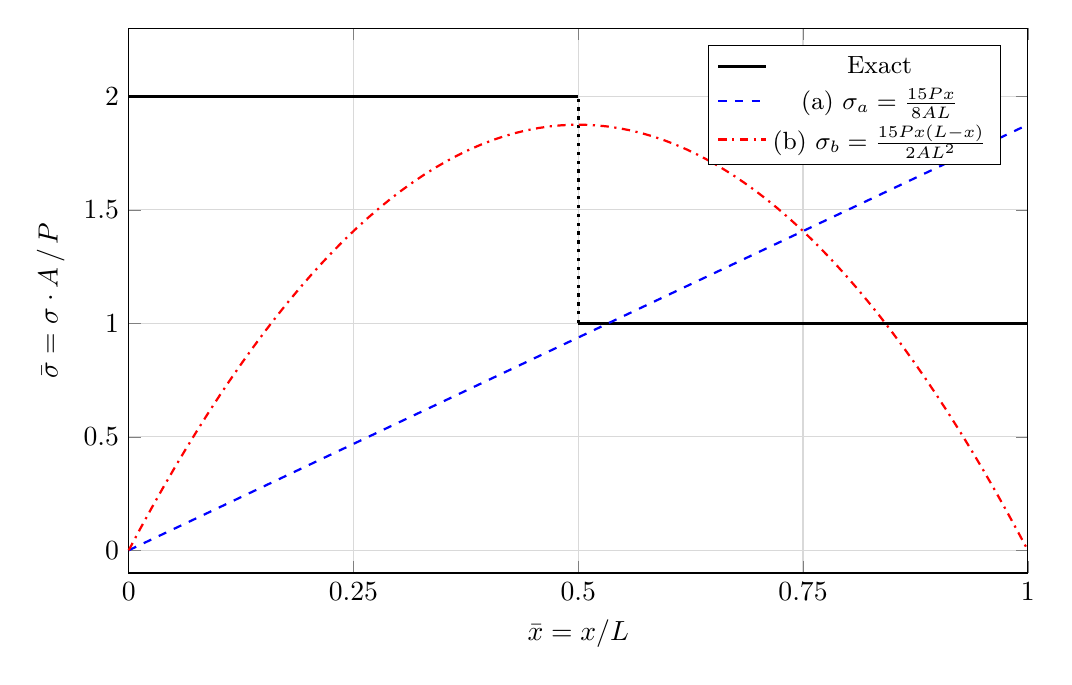
\begin{tikzpicture}
\begin{axis}[
    width=13cm, height=8.5cm,
    xlabel={$\bar{x} = x/L$},
    ylabel={$\bar{\sigma} = \sigma \cdot A \,/\, P$},
    xmin=0, xmax=1,
    ymin=-0.1, ymax=2.3,
    xtick={0, 0.25, 0.5, 0.75, 1.0},
    ytick={0, 0.5, 1.0, 1.5, 2.0},
    grid=major,
    grid style={gray!30},
    legend style={at={(0.97,0.97)}, anchor=north east, font=\small},
    every axis plot/.append style={thick},
    clip=false
]

% Exact solution (piecewise constant)
\addplot[black, very thick, solid, domain=0:0.5, samples=2] {2};
\addplot[black, very thick, solid, domain=0.5:1, samples=2, forget plot] {1};
% Vertical jump at x=L/2
\draw[black, very thick, dotted] (axis cs:0.5, 1) -- (axis cs:0.5, 2);
\addlegendentry{Exact}

% Part a) - one term (linear)
\addplot[blue, thick, dashed, domain=0:1, samples=2] {(15/8)*x};
\addlegendentry{(a) $\sigma_a = \frac{15Px}{8AL}$}

% Part b) - two terms (parabolic)
\addplot[red, thick, dashdotted, domain=0:1, samples=80] {(15/2)*x*(1-x)};
\addlegendentry{(b) $\sigma_b = \frac{15Px(L-x)}{2AL^2}$}

\end{axis}
\end{tikzpicture}
\caption{Non-dimensional stress fields: exact solution vs.\ one-term and two-term Rayleigh-Ritz approximations.}
\label{fig:stress}
\end{figure}

\begin{table}[H]
\centering
\renewcommand{\arraystretch}{1.4}
\begin{tabular}{@{}c c c c@{}}
\toprule
$\bar{x}$ & $\bar{\sigma}_{\text{exact}}$ & $\bar{\sigma}_a$ & $\bar{\sigma}_b$ \\
\midrule
$0$    & $2.000$ & $0$     & $0$     \\
$0.25$ & $2.000$ & $0.469$ & $1.406$ \\
$0.50^{-}$ & $2.000$ & $0.938$ & $1.875$ \\
$0.50^{+}$ & $1.000$ & $0.938$ & $1.875$ \\
$0.75$ & $1.000$ & $1.406$ & $1.406$ \\
$1.00$ & $1.000$ & $1.875$ & $0$     \\
\bottomrule
\end{tabular}
\caption{Stress comparison at key locations.}
\label{tab:stress}
\end{table}

% ======================================================================
\section{Discussion}\label{sec:discussion}
% ======================================================================

\subsection{Incomplete Trial Functions and Convergence}

Both trial functions in this problem \textbf{omit the linear term} $a_1 x$.  As discussed in Cook, Section~3.6, completeness of the polynomial basis requires that no lowest-order admissible terms be omitted.  The term $a_1 x$ represents the \textit{constant-strain capability}: it is the only term for which $u_{,x}$ is a nonzero constant.  Without it, the trial function is \textit{incomplete}, and convergence to the exact solution is not guaranteed even as more higher-order terms are added.

Concretely, for any trial function of the form $u(x) = a_2 x^2 + a_3 x^3 + \cdots + a_n x^n$, the strain is $\varepsilon(x) = u_{,x} = 2a_2 x + 3a_3 x^2 + \cdots$, which \textbf{always vanishes at $x=0$}.  This contradicts the exact solution, where $\sigma(0) = 2P/A$ is the \textit{maximum} stress in the bar.

\subsection{Overly Stiff Approximation}

The Rayleigh-Ritz method with displacement-based trial functions yields solutions that are \textit{either exact or too stiff} (Cook, Section~3.6).  The approximate displacement field imposes kinematic constraints that prevent the structure from deforming freely, creating an effectively stiffer substitute structure.  Our results confirm this:

\begin{itemize}
    \item \textbf{Part (a):}\; $u_a(L) = \frac{15PL}{16EA} \approx 0.938\,\frac{PL}{EA}$, while $u_{\text{exact}}(L) = \frac{3PL}{2EA} = 1.5\,\frac{PL}{EA}$.  The displacement is \textbf{underestimated by 37.5\%}.
    \item \textbf{Part (b):}\; $u_b(L) = \frac{5PL}{4EA} = 1.25\,\frac{PL}{EA}$, still \textbf{underestimated by 16.7\%}.
\end{itemize}

Adding the $a_3 x^3$ term provides one more degree of freedom, improving the result.  However, neither approximation can match the exact piecewise-linear displacement field because the basis lacks the $a_1 x$ term.

\subsection{Displacement Accuracy vs.\ Stress Accuracy}

Cook, Section~3.5 notes that \textit{approximate displacements are more accurate than approximate stresses}, because stresses are computed from \textit{derivatives} of the displacement field, which amplify discrepancies.  Our results illustrate this dramatically:

\begin{itemize}
    \item \textbf{Displacement:}\; Part~(b) is within 16.7\% of the exact value at $x = L$.
    \item \textbf{Stress:}\; At $x = 0$, both approximations give $\sigma = 0$, while the exact stress is $2P/A$ --- an error of \textbf{100\%}.  At $x = L$, part~(a) gives $\sigma_a(L) = 15P/(8A) = 1.875\,P/A$, \textbf{overestimating} the exact value $P/A$ by 87.5\%, while part~(b) gives $\sigma_b(L) = 0$, \textbf{underestimating} by 100\%.
\end{itemize}

This confirms that approximate stresses can be too high in some regions and too low in others, even when the displacements are uniformly underestimated.

\subsection{Physical Interpretation of the Plots}

From \cref{fig:displacement}:
\begin{itemize}
    \item The exact displacement is piecewise linear with a slope change at $x = L/2$ (where the concentrated load introduces a discontinuity in the internal force).
    \item Both polynomial approximations are smooth (no slope discontinuity), so they cannot capture the kink in the exact solution.
    \item The two-term approximation ($u_b$) is significantly closer to the exact solution, especially at $x = L$.
\end{itemize}

From \cref{fig:stress}:
\begin{itemize}
    \item The exact stress is piecewise constant with a jump from $2P/A$ to $P/A$ at $x = L/2$.
    \item Part~(a) gives a linearly increasing stress, completely missing the constant-stress nature of the solution.
    \item Part~(b) gives a parabolic stress that peaks at $x = L/2$ with $\sigma_b(L/2) = 15P/(8A) = 1.875\,P/A$, which is between the two exact values ($2P/A$ and $P/A$).  The two-term stress ``averages'' the jump rather than capturing it.
    \item Both approximations give $\sigma(0) = 0$, which is a direct consequence of the missing $a_1 x$ term.
\end{itemize}

\subsection{Effect of Restoring the Linear Term}

If the trial function were $u(x) = a_1 x + a_2 x^2 + a_3 x^3$ (a complete cubic), the basis would be able to capture the constant-strain mode, and the Rayleigh-Ritz approximation would satisfy $\varepsilon(0) \neq 0$.  The solution would be significantly improved, with much better stress predictions near the fixed end.  This underscores Cook's observation that \textit{completeness demands that the lowest-order admissible terms be included}.

% ######################################################################
%  QUESTION 2
% ######################################################################
\newpage
% ======================================================================
\section{Problem 2: Bilinear Rectangular Finite Element}\label{sec:q2}
% ======================================================================

Derive $u_i(s,t)$ for a $2a\times 2b$ rectangular element.  Einstein summation implied; $i,j,k,l\in\{1,2\}$; $I,J\in\{1,2,3,4\}$; $r\in\{1,2,3,4\}$; $(\cdot)_{,j}=\partial(\cdot)/\partial x_j$, $x_1\equiv s$, $x_2\equiv t$.

\begin{figure}[H]
\centering
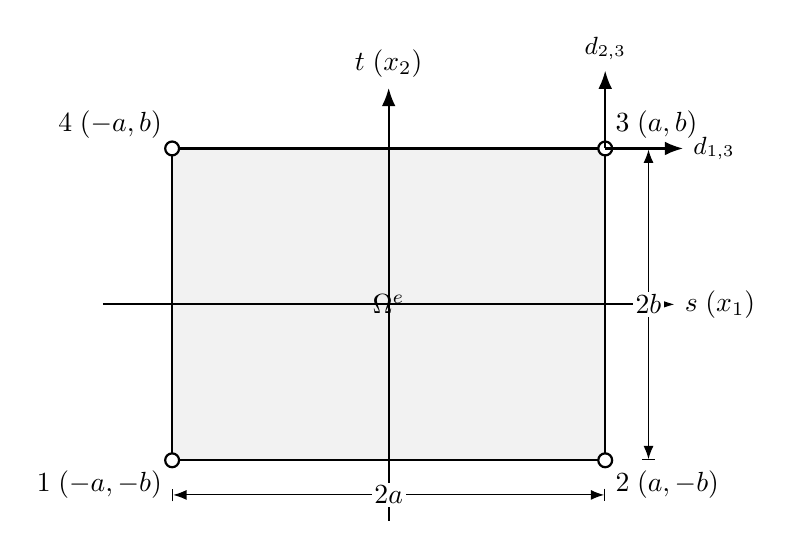
\begin{tikzpicture}[>=Latex, font=\sffamily, scale=1.1]
    % Element
    \draw[thick, fill=black!5] (-2.5,-1.8) rectangle (2.5,1.8);
    % Axes
    \draw[->,thick] (-3.3,0) -- (3.3,0) node[right]{$s\;(x_1)$};
    \draw[->,thick] (0,-2.5) -- (0,2.5) node[above]{$t\;(x_2)$};
    % Nodes
    \filldraw[fill=white, draw=black, thick] (-2.5,-1.8) circle (0.08)
        node[below left]{$1\;(-a,-b)$};
    \filldraw[fill=white, draw=black, thick] (2.5,-1.8) circle (0.08)
        node[below right]{$2\;(a,-b)$};
    \filldraw[fill=white, draw=black, thick] (2.5,1.8) circle (0.08)
        node[above right]{$3\;(a,b)$};
    \filldraw[fill=white, draw=black, thick] (-2.5,1.8) circle (0.08)
        node[above left]{$4\;(-a,b)$};
    % DOF arrows at node 3
    \draw[->,thick,black] (2.5,1.8) -- (3.4,1.8) node[right]{\small $d_{1,3}$};
    \draw[->,thick,black] (2.5,1.8) -- (2.5,2.7) node[above]{\small $d_{2,3}$};
    % Dimensions
    \draw[|<->|,thin] (-2.5,-2.2) -- (2.5,-2.2) node[midway, fill=white, inner sep=1pt]{$2a$};
    \draw[|<->|,thin] (3.0,-1.8) -- (3.0,1.8) node[midway, fill=white, inner sep=1pt]{$2b$};
    % Omega label
    \node at (0,0) {$\Omega^e$};
\end{tikzpicture}
\caption{Rectangular element $\Omega^e=[-a,a]\times[-b,b]$; nodes numbered counter-clockwise.  Each node carries two displacement DOFs $d_{iI}$.}
\label{fig:rect}
\end{figure}

\subsection{Potential Energy and Rayleigh-Ritz Equations}

Let $\varepsilon_{ij}=\tfrac{1}{2}(u_{i,j}+u_{j,i})$, $\sigma_{ij}=C_{ijkl}\,\varepsilon_{kl}$, with $C_{ijkl}=C_{jikl}=C_{ijlk}=C_{klij}$.
\begin{equation}\label{eq:pi2d}
\Pi_p[u_i]=\frac{1}{2}\int_\Omega C_{ijkl}\,u_{i,j}\,u_{k,l}\,d\Omega
-\int_\Omega f_i\,u_i\,d\Omega
-\int_{\Gamma_N}\!\bar{t}_i\,u_i\,d\Gamma
\end{equation}

Let $u_i^h=N_I\,d_{iI}$, $\varepsilon_{ij}^h=\tfrac{1}{2}(N_{I,j}\,d_{iI}+N_{I,i}\,d_{jI})$.  Stationarity $\partial\Pi_p/\partial d_{iI}=0$ gives
\begin{equation}\label{eq:elem_eq}
K_{iI,kJ}\;d_{kJ}=F_{iI}
\end{equation}
\begin{equation}\label{eq:KF2d}
K_{iI,kJ}=\int_{\Omega^e}C_{ijkl}\,N_{I,j}\,N_{J,l}\;d\Omega,\qquad
F_{iI}=\int_{\Omega^e}f_i\,N_I\;d\Omega+\int_{\Gamma_N^e}\bar{t}_i\,N_I\;d\Gamma
\end{equation}

\subsection{Derivation of the Shape Functions}

\paragraph{Polynomial basis.}
$p_r(s,t)$: $p_1=1$, $p_2=s$, $p_3=t$, $p_4=st$ (4 monomials, 4 nodes).

\paragraph{Field approximation.}
Let $u_i(s,t)=p_r\,\alpha_{ir}$.  At node $I$:
\[
d_{iI}=p_r(s_I,t_I)\,\alpha_{ir}=A_{Ir}\,\alpha_{ir}
\]
where $A_{Ir}:=p_r(s_I,t_I)$:
\begin{equation}\label{eq:Amat}
[A_{Ir}]=
\begin{bmatrix}
p_1(s_1,t_1) & p_2(s_1,t_1) & p_3(s_1,t_1) & p_4(s_1,t_1)\\
p_1(s_2,t_2) & p_2(s_2,t_2) & p_3(s_2,t_2) & p_4(s_2,t_2)\\
p_1(s_3,t_3) & p_2(s_3,t_3) & p_3(s_3,t_3) & p_4(s_3,t_3)\\
p_1(s_4,t_4) & p_2(s_4,t_4) & p_3(s_4,t_4) & p_4(s_4,t_4)
\end{bmatrix}
=
\begin{bmatrix}
1 & -a & -b &  ab\\
1 &  a & -b & -ab\\
1 &  a &  b &  ab\\
1 & -a &  b & -ab
\end{bmatrix}.
\end{equation}

\paragraph{Inversion.}
$\alpha_{ir}=(A^{-1})_{rI}\,d_{iI}$.  Row-reduce $[A\mid\mathbf{I}_4]$:
\begin{gather*}
R_2\leftarrow R_2-R_1,\quad
R_3\leftarrow R_3-R_1,\quad
R_4\leftarrow R_4-R_1
\\[2pt]\longrightarrow\quad
\begin{bmatrix}
1 & -a & -b &  ab\\
0 &  2a & 0 & -2ab\\
0 &  2a & 2b & 0\\
0 &  0  & 2b & -2ab
\end{bmatrix}
\\[6pt]
R_3\leftarrow R_3-R_2,\qquad R_4\leftarrow R_4-R_3
\\[2pt]\longrightarrow\quad
\begin{bmatrix}
1 & -a & -b &  ab\\
0 &  2a & 0 & -2ab\\
0 &  0  & 2b & 2ab\\
0 &  0  & 0  & -4ab
\end{bmatrix}
\end{gather*}
Hence $\det[A]=1\cdot 2a\cdot 2b\cdot(-4ab)=-16a^2b^2\neq 0$.  Back-substituting:
\begin{equation}\label{eq:Ainv}
[(A^{-1})_{rI}]=\frac{1}{4}
\begin{bmatrix}
 1       &  1       &  1       &  1      \\[3pt]
-\dfrac{1}{a} &  \dfrac{1}{a} &  \dfrac{1}{a} & -\dfrac{1}{a}\\[6pt]
-\dfrac{1}{b} & -\dfrac{1}{b} &  \dfrac{1}{b} &  \dfrac{1}{b}\\[6pt]
 \dfrac{1}{ab}& -\dfrac{1}{ab}&  \dfrac{1}{ab}& -\dfrac{1}{ab}
\end{bmatrix}
\end{equation}

\textit{Check:}\; $A_{1r}(A^{-1})_{r1}=\tfrac{1}{4}+\tfrac{1}{4}+\tfrac{1}{4}+\tfrac{1}{4}=1$,\; $A_{1r}(A^{-1})_{r2}=\tfrac{1}{4}-\tfrac{1}{4}+\tfrac{1}{4}-\tfrac{1}{4}=0$.\; $\Rightarrow\;A_{Ir}(A^{-1})_{rJ}=\delta_{IJ}$.\;\checkmark

\paragraph{Shape functions.}
$u_i=p_r\,(A^{-1})_{rI}\,d_{iI}=N_I\,d_{iI}$, where $N_I=p_r(A^{-1})_{rI}$.  Column by column:

\medskip\noindent$I=1$:
\begin{align*}
N_1 &= [1,\;s,\;t,\;st]\;\frac{1}{4}\!\begin{Bmatrix}1\\-1/a\\-1/b\\1/(ab)\end{Bmatrix}
     = \frac{1}{4}\!\left(1-\frac{s}{a}-\frac{t}{b}+\frac{st}{ab}\right) \\[4pt]
    &= \frac{1}{4ab}\big(ab-sb-at+st\big)
     = \frac{(a-s)(b-t)}{4ab}
\end{align*}

\noindent$I=2$:
\begin{align*}
N_2 &= [1,\;s,\;t,\;st]\;\frac{1}{4}\!\begin{Bmatrix}1\\1/a\\-1/b\\-1/(ab)\end{Bmatrix}
     = \frac{1}{4}\!\left(1+\frac{s}{a}-\frac{t}{b}-\frac{st}{ab}\right) \\[4pt]
    &= \frac{1}{4ab}\big(ab+sb-at-st\big)
     = \frac{(a+s)(b-t)}{4ab}
\end{align*}

\noindent$I=3$:
\begin{align*}
N_3 &= [1,\;s,\;t,\;st]\;\frac{1}{4}\!\begin{Bmatrix}1\\1/a\\1/b\\1/(ab)\end{Bmatrix}
     = \frac{1}{4}\!\left(1+\frac{s}{a}+\frac{t}{b}+\frac{st}{ab}\right) \\[4pt]
    &= \frac{1}{4ab}\big(ab+sb+at+st\big)
     = \frac{(a+s)(b+t)}{4ab}
\end{align*}

\noindent$I=4$:
\begin{align*}
N_4 &= [1,\;s,\;t,\;st]\;\frac{1}{4}\!\begin{Bmatrix}1\\-1/a\\1/b\\-1/(ab)\end{Bmatrix}
     = \frac{1}{4}\!\left(1-\frac{s}{a}+\frac{t}{b}-\frac{st}{ab}\right) \\[4pt]
    &= \frac{1}{4ab}\big(ab-sb+at-st\big)
     = \frac{(a-s)(b+t)}{4ab}
\end{align*}

\paragraph{Compact form.}
Let $\xi_I:=s_I/a\in\{-1,+1,+1,-1\}$, $\eta_I:=t_I/b\in\{-1,-1,+1,+1\}$:
\begin{equation}\label{eq:NI}
\boxed{N_I(s,t)=\frac{(a+\xi_I\,s)(b+\eta_I\,t)}{4ab}=\frac{1}{4}\!\left(1+\xi_I\frac{s}{a}\right)\!\!\left(1+\eta_I\frac{t}{b}\right)}
\end{equation}

Explicitly:
\begin{equation}\label{eq:NI_explicit}
N_1=\frac{(a-s)(b-t)}{4ab},\quad
N_2=\frac{(a+s)(b-t)}{4ab},\quad
N_3=\frac{(a+s)(b+t)}{4ab},\quad
N_4=\frac{(a-s)(b+t)}{4ab}.
\end{equation}

\paragraph{Kronecker-delta.}
$s_J=\xi_J a$, $t_J=\eta_J b$:
\[
N_I(s_J,t_J)=\frac{(1+\xi_I\xi_J)(1+\eta_I\eta_J)}{4}
=\begin{cases}1 & I=J\;\;(\xi_I\xi_J=\eta_I\eta_J=1)\\0 & I\neq J\;\;(\text{at least one factor vanishes})\end{cases}
=\delta_{IJ}.\;\checkmark
\]

\paragraph{Partition of unity.}
\begin{align*}
\sum_{I=1}^{4}N_I
&= \frac{1}{4}\sum_{I=1}^{4}\!\left(1+\xi_I\frac{s}{a}\right)\!\!\left(1+\eta_I\frac{t}{b}\right) \\[6pt]
&= \frac{1}{4}\sum_{I=1}^{4}\!\left[1+\xi_I\frac{s}{a}+\eta_I\frac{t}{b}+\xi_I\eta_I\frac{st}{ab}\right] \\[6pt]
&= \frac{1}{4}\!\left[\underbrace{\sum_I 1}_{=4}
  +\frac{s}{a}\underbrace{\sum_I\xi_I}_{-1+1+1-1=0}
  +\frac{t}{b}\underbrace{\sum_I\eta_I}_{-1-1+1+1=0}
  +\frac{st}{ab}\underbrace{\sum_I\xi_I\eta_I}_{1-1+1-1=0}\right] \\[6pt]
&= \frac{1}{4}\cdot 4 = 1
\end{align*}
\begin{equation}\label{eq:pou}
\sum_{I=1}^{4}N_I(s,t)=1\qquad\forall\;(s,t)\in\Omega^e.\;\checkmark
\end{equation}

\subsection{Displacement Interpolation}
\begin{equation}\label{eq:disp_interp}
\boxed{u_i(s,t)=N_I(s,t)\;d_{iI}=\frac{(a+\xi_I\,s)(b+\eta_I\,t)}{4ab}\;d_{iI},\qquad i\in\{1,2\},\;I\;\text{summed}\;1\text{--}4}
\end{equation}

Expanded ($u\equiv u_1$, $v\equiv u_2$):
\begin{equation}\label{eq:uv_expanded}
\begin{aligned}
u(s,t) &= N_1\,u_1 + N_2\,u_2 + N_3\,u_3 + N_4\,u_4\\
v(s,t) &= N_1\,v_1 + N_2\,v_2 + N_3\,v_3 + N_4\,v_4
\end{aligned}
\end{equation}

Matrix form ($\{\mathbf{d}\}=\{u_1,v_1,u_2,v_2,u_3,v_3,u_4,v_4\}^T$):
\begin{equation}\label{eq:Nmat}
\begin{Bmatrix}u\\v\end{Bmatrix}=
\underbrace{\begin{bmatrix}
N_1 & 0 & N_2 & 0 & N_3 & 0 & N_4 & 0\\
0 & N_1 & 0 & N_2 & 0 & N_3 & 0 & N_4
\end{bmatrix}}_{[\mathbf{N}]\;(2\times 8)}\{\mathbf{d}\}
\end{equation}

\subsection{Strain--Displacement Relation and Element Stiffness}

Gradients:
\begin{equation}\label{eq:NI_grad}
N_{I,1}=\frac{\partial N_I}{\partial s}=\frac{\xi_I(b+\eta_I t)}{4ab},\qquad
N_{I,2}=\frac{\partial N_I}{\partial t}=\frac{\eta_I(a+\xi_I s)}{4ab}.
\end{equation}

In Voigt notation $\{\boldsymbol{\varepsilon}\}=\{\varepsilon_{11},\varepsilon_{22},2\varepsilon_{12}\}^T=[\mathbf{B}]\{\mathbf{d}\}$, the $3\times 2$ sub-block for node $I$:
\begin{equation}\label{eq:BI}
[\mathbf{B}_I]=
\begin{bmatrix}
N_{I,1} & 0\\
0 & N_{I,2}\\
N_{I,2} & N_{I,1}
\end{bmatrix}
=\frac{1}{4ab}
\begin{bmatrix}
\xi_I(b+\eta_I t) & 0\\
0 & \eta_I(a+\xi_I s)\\
\eta_I(a+\xi_I s) & \xi_I(b+\eta_I t)
\end{bmatrix}
\end{equation}
$[\mathbf{B}]=[\mathbf{B}_1\;\mathbf{B}_2\;\mathbf{B}_3\;\mathbf{B}_4]$ ($3\times 8$, varies linearly in $s,t$).  Element stiffness ($h=1$):
\begin{equation}\label{eq:ke}
[\mathbf{k}^e]=\int_{\Omega^e}[\mathbf{B}]^T[\mathbf{C}][\mathbf{B}]\;dA
=\int_{-b}^{b}\!\int_{-a}^{a}[\mathbf{B}]^T[\mathbf{C}][\mathbf{B}]\;ds\,dt
\end{equation}
In index notation:
\begin{equation}\label{eq:ke_index}
k_{iI,kJ}=\int_{-b}^{b}\!\int_{-a}^{a}C_{ijkl}\;N_{I,j}(s,t)\;N_{J,l}(s,t)\;ds\,dt.
\end{equation}
This is the $8\times 8$ element stiffness for the $2a\times 2b$ bilinear rectangle.

\subsection{Natural (Isoparametric) Coordinates}\label{sec:natural}

\paragraph{Coordinate mapping.}
Let $\hat{\Omega}=[-1,1]^2$ (parent domain).  Map to $\Omega^e$:
\begin{equation}\label{eq:map}
s = a\,\zeta,\qquad t = b\,\eta
\end{equation}
so that
\[
\zeta=\frac{s}{a}\in[-1,1],\qquad \eta=\frac{t}{b}\in[-1,1].
\]
Nodes: $(\zeta_I,\eta_I)=(\xi_I,\eta_I)=\{(-1,-1),(+1,-1),(+1,+1),(-1,+1)\}$.

\paragraph{Jacobian.}
\begin{equation}\label{eq:J}
[\mathbf{J}]=
\begin{bmatrix}
\dfrac{\partial s}{\partial\zeta} & \dfrac{\partial t}{\partial\zeta} \\[10pt]
\dfrac{\partial s}{\partial\eta}  & \dfrac{\partial t}{\partial\eta}
\end{bmatrix}
=\begin{bmatrix} a & 0 \\ 0 & b \end{bmatrix}
\end{equation}
\begin{equation}\label{eq:detJ}
\det[\mathbf{J}]=a\cdot b - 0\cdot 0 = ab
\end{equation}
\begin{equation}\label{eq:Jinv}
[\mathbf{J}]^{-1}=\frac{1}{ab}\begin{bmatrix}b & 0\\0 & a\end{bmatrix}
=\begin{bmatrix}1/a & 0\\0 & 1/b\end{bmatrix}
\end{equation}

\paragraph{Shape functions in $(\zeta,\eta)$.}
\begin{equation}\label{eq:NI_nat}
\boxed{\hat{N}_I(\zeta,\eta)=\frac{1}{4}(1+\xi_I\,\zeta)(1+\eta_I\,\eta)}
\end{equation}

Explicitly:
\begin{align*}
\hat{N}_1 &= \tfrac{1}{4}(1-\zeta)(1-\eta) \\[3pt]
\hat{N}_2 &= \tfrac{1}{4}(1+\zeta)(1-\eta) \\[3pt]
\hat{N}_3 &= \tfrac{1}{4}(1+\zeta)(1+\eta) \\[3pt]
\hat{N}_4 &= \tfrac{1}{4}(1-\zeta)(1+\eta)
\end{align*}

\paragraph{Equivalence.}
$\zeta=s/a$, $\eta=t/b$:
\begin{align*}
\hat{N}_I\!\left(\frac{s}{a},\frac{t}{b}\right)
&= \frac{1}{4}\!\left(1+\xi_I\frac{s}{a}\right)\!\!\left(1+\eta_I\frac{t}{b}\right) \\[6pt]
&= \frac{1}{4}\cdot\frac{a+\xi_I s}{a}\cdot\frac{b+\eta_I t}{b}
 = \frac{(a+\xi_I s)(b+\eta_I t)}{4ab}
 = N_I(s,t)\;\;\checkmark
\end{align*}

\paragraph{Gradient transformation.}
\begin{equation}\label{eq:grad_transform}
\begin{Bmatrix}
\dfrac{\partial N_I}{\partial s} \\[10pt]
\dfrac{\partial N_I}{\partial t}
\end{Bmatrix}
= [\mathbf{J}]^{-1}
\begin{Bmatrix}
\dfrac{\partial \hat{N}_I}{\partial\zeta} \\[10pt]
\dfrac{\partial \hat{N}_I}{\partial\eta}
\end{Bmatrix}
\end{equation}

Parent-domain derivatives: $\partial\hat{N}_I/\partial\zeta=\xi_I(1+\eta_I\eta)/4$, $\partial\hat{N}_I/\partial\eta=\eta_I(1+\xi_I\zeta)/4$.  Applying $[\mathbf{J}]^{-1}$:
\begin{align*}
\frac{\partial N_I}{\partial s}
&= \frac{1}{a}\cdot\frac{\xi_I}{4}(1+\eta_I\eta)
 = \frac{\xi_I(1+\eta_I\eta)}{4a}
 = \frac{\xi_I(b+\eta_I t)}{4ab}\;\;\checkmark \\[6pt]
\frac{\partial N_I}{\partial t}
&= \frac{1}{b}\cdot\frac{\eta_I}{4}(1+\xi_I\zeta)
 = \frac{\eta_I(1+\xi_I\zeta)}{4b}
 = \frac{\eta_I(a+\xi_I s)}{4ab}\;\;\checkmark
\end{align*}
These match \cref{eq:NI_grad} exactly.

\paragraph{Stiffness in $(\zeta,\eta)$.}
$ds\,dt=ab\,d\zeta\,d\eta$:
\begin{equation}\label{eq:ke_nat}
[\mathbf{k}^e]=\int_{-1}^{1}\!\int_{-1}^{1}[\mathbf{B}(\zeta,\eta)]^T\,[\mathbf{C}]\,[\mathbf{B}(\zeta,\eta)]\;\det[\mathbf{J}]\;d\zeta\,d\eta
\end{equation}

$\det[\mathbf{J}]=ab$ is constant:
\begin{equation}\label{eq:ke_nat2}
[\mathbf{k}^e]=ab\int_{-1}^{1}\!\int_{-1}^{1}[\mathbf{B}(\zeta,\eta)]^T\,[\mathbf{C}]\,[\mathbf{B}(\zeta,\eta)]\;d\zeta\,d\eta
\end{equation}

$2\times 2$ Gauss quadrature ($\zeta_g,\eta_g=\pm 1/\sqrt{3}$, $w_g=1$) integrates exactly:
\begin{equation}\label{eq:ke_gauss}
[\mathbf{k}^e]=ab\sum_{g=1}^{4}w_g\;[\mathbf{B}(\zeta_g,\eta_g)]^T\,[\mathbf{C}]\,[\mathbf{B}(\zeta_g,\eta_g)]
\end{equation}

In practice: work in $(\zeta,\eta)$, never form $[A]^{-1}$, evaluate via Gauss quadrature.

\subsection{Discussion of Problem 2}

The shape functions in \cref{eq:NI} have a tensor-product structure: $N_I(s,t)=L^{(s)}_{m(I)}(s)\;L^{(t)}_{n(I)}(t)$, where $L^{(s)}_1=(a-s)/(2a)$, $L^{(s)}_2=(a+s)/(2a)$ are the 1-D linear shape functions in $s$, and similarly for $t$.  This is a direct extension of the bar element interpolation (Cook, Section~3.8, Eq.~3.8-8) into two dimensions.

The bilinear basis $\{1,s,t,st\}$ is \textit{complete to degree 1} in Pascal's triangle (all terms with $s^m t^n$, $m+n\le 1$, are present), plus the cross-term $st$.  Completeness to degree 1 guarantees constant-strain (and hence constant-stress) capability: any state $u_i=a_i+b_{ij}x_j$ with constant $b_{ij}$ can be represented exactly.  The partition-of-unity property ($\sum N_I=1$) ensures that rigid-body translations are contained in the approximation space.

The strain--displacement matrix $[\mathbf{B}]$ is not constant over $\Omega^e$; it varies linearly in $s$ and $t$.  This is a key difference from the 1-D bar, where $[\mathbf{B}]$ is constant.  As a consequence, the integrand of the stiffness integral \cref{eq:ke} is quadratic in $s$ and $t$, and the analytical evaluation requires integration of polynomial terms up to $s^2t^2$ over the rectangular domain --- possible in closed form, but often delegated to $2\times 2$ Gauss quadrature in practice.

The element has 8 DOFs and 3 independent strain components, so the system is well-posed.  It possesses 3 rigid-body modes ($u$-translation, $v$-translation, and in-plane rotation for small angles) and 5 deformation modes, consistent with $\mathrm{rank}([\mathbf{k}^e])=5$.

% ======================================================================
\section{Numerical Validation}\label{sec:validation}
% ======================================================================

The Rayleigh-Ritz solutions from Question~1 and the element stiffness from Question~2 are validated against two independent FEM implementations: \textbf{OpenSees} (via \texttt{openseespy}) and \textbf{FemLab-Python} (in-house FEM library).

\subsection{OpenSees Validation --- Question 1}

A 1-D bar with 20 linear truss elements ($\Delta x=L/20$) is modelled in OpenSees with the same loading ($P$ at $x=L/2$ and $x=L$) and boundary condition ($u(0)=0$).  Since the exact displacement is piecewise linear, the linear FEM solution coincides with the exact solution to machine precision.

\begin{table}[H]
\centering
\renewcommand{\arraystretch}{1.3}
\begin{tabular}{@{}c S[table-format=1.4] S[table-format=1.4] S[table-format=1.4] S[table-format=1.4] S[table-format=1.3]@{}}
\toprule
{$\bar{x}$} & {Exact} & {OpenSees} & {RR (a)} & {RR (b)} & {FEM err (\%)} \\
\midrule
0.00 & 0.0000 & 0.0000 & 0.0000 & 0.0000 & 0.000 \\
0.25 & 0.5000 & 0.5000 & 0.0586 & 0.1953 & 0.000 \\
0.50 & 1.0000 & 1.0000 & 0.2344 & 0.6250 & 0.000 \\
0.75 & 1.2500 & 1.2500 & 0.5273 & 1.0547 & 0.000 \\
1.00 & 1.5000 & 1.5000 & 0.9375 & 1.2500 & 0.000 \\
\bottomrule
\end{tabular}
\caption{Normalised displacement $\bar{u}=u\cdot EA/(PL)$: OpenSees FEM vs.\ exact and Rayleigh-Ritz.}
\label{tab:opensees_disp}
\end{table}

\begin{table}[H]
\centering
\renewcommand{\arraystretch}{1.3}
\begin{tabular}{@{}c S[table-format=1.4] S[table-format=1.4] S[table-format=1.4] S[table-format=1.4]@{}}
\toprule
{$\bar{x}$} & {Exact} & {OpenSees} & {RR (a)} & {RR (b)} \\
\midrule
0.00 & 2.0000 & 2.0000 & 0.0000 & 0.0000 \\
0.25 & 2.0000 & 2.0000 & 0.4688 & 1.4062 \\
0.50 & 2.0000 & 2.0000 & 0.9375 & 1.8750 \\
0.75 & 1.0000 & 1.0000 & 1.4062 & 1.4062 \\
1.00 & 1.0000 & 1.0000 & 1.8750 & 0.0000 \\
\bottomrule
\end{tabular}
\caption{Normalised stress $\bar{\sigma}=\sigma\cdot A/P$: OpenSees FEM vs.\ exact and Rayleigh-Ritz.}
\label{tab:opensees_stress}
\end{table}

The FEM solution matches the exact solution with $\max|u_\text{FEM}-u_\text{exact}|=\mathcal{O}(10^{-14})$, confirming both the exact solution derivation and the FEM implementation.  The large discrepancies between the Rayleigh-Ritz approximations and the FEM/exact results --- particularly for stress near $x=0$ --- are a direct consequence of the missing $a_1 x$ term discussed in \cref{sec:discussion}.

\subsection{FemLab Validation --- Question 1}

The same 1-D bar problem is solved using the FemLab-Python library (\texttt{kbar} element) with 20 elements.

\begin{table}[H]
\centering
\renewcommand{\arraystretch}{1.3}
\begin{tabular}{@{}c S[table-format=1.4] S[table-format=1.4] S[table-format=1.4] S[table-format=1.4] S[table-format=1.3]@{}}
\toprule
{$\bar{x}$} & {Exact} & {FemLab} & {RR (a)} & {RR (b)} & {FEM err (\%)} \\
\midrule
0.00 & 0.0000 & 0.0000 & 0.0000 & 0.0000 & 0.000 \\
0.25 & 0.5000 & 0.5000 & 0.0586 & 0.1953 & 0.000 \\
0.50 & 1.0000 & 1.0000 & 0.2344 & 0.6250 & 0.000 \\
0.75 & 1.2500 & 1.2500 & 0.5273 & 1.0547 & 0.000 \\
1.00 & 1.5000 & 1.5000 & 0.9375 & 1.2500 & 0.000 \\
\bottomrule
\end{tabular}
\caption{Normalised displacement: FemLab vs.\ exact and Rayleigh-Ritz.}
\label{tab:femlab_disp}
\end{table}

FemLab results are identical to OpenSees and to the exact solution, providing independent cross-validation.

\subsection{FemLab Validation --- Question 2}

The element stiffness matrix $[\mathbf{k}^e]$ for a single $2\times 2$ plane-stress Q4 element ($E=100$, $\nu=0.3$, $h=1$) is computed using FemLab's \texttt{keq4e} routine and compared against the analytical $2\times 2$ Gauss quadrature result from \cref{eq:ke_nat2}:

\begin{table}[H]
\centering
\renewcommand{\arraystretch}{1.3}
\begin{tabular}{@{}l r@{}}
\toprule
\textbf{Check} & \textbf{Result} \\
\midrule
$\|[\mathbf{k}^e]_\text{FemLab}-[\mathbf{k}^e]_\text{analytical}\|$ & $2.76\times 10^{-14}$ \\
Relative error & $1.43\times 10^{-16}$ \\
Zero eigenvalues (rigid-body modes) & 3 \\
Positive eigenvalues (deformation modes) & 5 \\
$\mathrm{rank}([\mathbf{k}^e])$ & 5 \\
$\|[\mathbf{k}^e]\,\mathbf{d}_\text{rigid}\|$ & $1.33\times 10^{-14}$ \\
\bottomrule
\end{tabular}
\caption{FemLab element stiffness verification for the $2a\times 2b$ bilinear rectangle.}
\label{tab:femlab_q2}
\end{table}

The FemLab Q4 element stiffness matches the analytical Gauss-quadrature result to machine precision.  The eigenvalue analysis confirms the expected rank of 5 (three rigid-body modes in 2-D: two translations and one rotation) and five independent deformation modes.

% ======================================================================
\section{Convergence Study: \texorpdfstring{$n$}{n}-Term Polynomial}\label{sec:convergence}
% ======================================================================

\subsection{Function Space and Admissibility}

Let $\mathcal{V}$ be the space of kinematically admissible displacement fields:
\begin{equation}\label{eq:V_space}
\mathcal{V}=\bigl\{v\in H^1(0,L)\;:\;v(0)=0\bigr\}
\end{equation}
where $H^1(0,L)$ is the Sobolev space of functions with square-integrable first derivatives,
equipped with the \emph{energy inner product}
\begin{equation}\label{eq:energy_ip}
\langle u,v\rangle_E = EA\int_0^L u_{,x}\,v_{,x}\,dx
\end{equation}
and the induced \emph{energy norm} $\|u\|_E=\sqrt{\langle u,u\rangle_E}$.

\subsection{General \texorpdfstring{$n$}{n}-Term Trial Function}

Let the $n$-dimensional trial subspace $\mathcal{V}^h_n\subset\mathcal{V}$ be spanned by the monomial basis
\begin{equation}\label{eq:basis_gen}
\phi_i(x)=x^{i+1},\qquad i=1,2,\dots,n
\end{equation}
so that the index $i$ labels the \emph{basis function number} while the
polynomial degree is $i+1$.  Every $\phi_i$ satisfies the essential BC
$\phi_i(0)=0$.  Note: $\phi_1=x^2$, corresponding to parts~(a)--(b);
the linear term $x^1$ remains \textbf{omitted}.

The trial displacement is
\begin{equation}\label{eq:u_gen}
u^h(x)=\sum_{i=1}^{n}a_i\,\phi_i(x)
       =a_1\,x^2 + a_2\,x^3 + \cdots + a_n\,x^{n+1},
\qquad a_i\in\mathbb{R}
\end{equation}
and the corresponding strain:
\begin{equation}\label{eq:eps_gen}
\varepsilon^h(x)=u^h_{,x}=\sum_{i=1}^{n}a_i\,\phi_i'(x)
               =2\,a_1\,x + 3\,a_2\,x^2 + \cdots + (n{+}1)\,a_n\,x^n
\end{equation}

\subsection{Total Potential Energy}

Substituting \cref{eq:u_gen} into the functional \cref{eq:pi}:

\paragraph{Strain energy.}
\begin{align}
U &= \frac{EA}{2}\int_0^L \bigl(u^h_{,x}\bigr)^2\,dx
   = \frac{EA}{2}\int_0^L
     \left(\sum_{i=1}^n a_i\,(i{+}1)\,x^i\right)
     \left(\sum_{j=1}^n a_j\,(j{+}1)\,x^j\right) dx \notag\\[6pt]
  &= \frac{EA}{2}\sum_{i=1}^n\sum_{j=1}^n
     a_i\,a_j\,(i{+}1)(j{+}1)
     \int_0^L x^{i+j}\,dx \notag\\[6pt]
  &= \frac{EA}{2}\sum_{i=1}^n\sum_{j=1}^n
     a_i\,a_j\,(i{+}1)(j{+}1)
     \cdot\frac{L^{i+j+1}}{i+j+1} \notag\\[6pt]
  &= \frac{1}{2}
     \begin{Bmatrix}a_1 & a_2 & \cdots & a_n\end{Bmatrix}
     \begin{bmatrix}
     K_{11} & K_{12} & \cdots & K_{1n}\\
     K_{21} & K_{22} & \cdots & K_{2n}\\
     \vdots & \vdots & \ddots & \vdots\\
     K_{n1} & K_{n2} & \cdots & K_{nn}
     \end{bmatrix}
     \begin{Bmatrix}a_1 \\ a_2 \\ \vdots \\ a_n\end{Bmatrix}
     \label{eq:U_gen}
\end{align}

\paragraph{Identification of the stiffness matrix $[\mathbf{K}]$.}
The $(i,j)$ entry of the $n\times n$ stiffness matrix is read off from \cref{eq:U_gen}:
\begin{equation}\label{eq:Kab_gen}
\boxed{K_{ij}
  = EA\,\frac{(i+1)(j+1)}{i+j+1}\,L^{i+j+1},
  \qquad i,j=1,2,\dots,n}
\end{equation}

In full matrix form:
\begin{equation}\label{eq:Kmat_full}
[\mathbf{K}] = EA
\begin{bmatrix}
\dfrac{2\cdot 2}{3}\,L^3 & \dfrac{2\cdot 3}{4}\,L^4 & \dfrac{2\cdot 4}{5}\,L^5 & \cdots & \dfrac{2(n{+}1)}{n{+}2}\,L^{n+2}\\[10pt]
\dfrac{3\cdot 2}{4}\,L^4 & \dfrac{3\cdot 3}{5}\,L^5 & \dfrac{3\cdot 4}{6}\,L^6 & \cdots & \dfrac{3(n{+}1)}{n{+}3}\,L^{n+3}\\[10pt]
\dfrac{4\cdot 2}{5}\,L^5 & \dfrac{4\cdot 3}{6}\,L^6 & \dfrac{4\cdot 4}{7}\,L^7 & \cdots & \dfrac{4(n{+}1)}{n{+}4}\,L^{n+4}\\[10pt]
\vdots & \vdots & \vdots & \ddots & \vdots \\[6pt]
\dfrac{(n{+}1)\cdot 2}{n{+}2}\,L^{n+2} & \dfrac{(n{+}1)\cdot 3}{n{+}3}\,L^{n+3} & \dfrac{(n{+}1)\cdot 4}{n{+}4}\,L^{n+4} & \cdots & \dfrac{(n{+}1)^2}{2n{+}1}\,L^{2n+1}
\end{bmatrix}
\end{equation}

\paragraph{Symmetry check.}  Exchanging $i\leftrightarrow j$:
$K_{ji}=EA\,\frac{(j+1)(i+1)}{j+i+1}\,L^{j+i+1}
=K_{ij}\;\checkmark$
\quad$\Longrightarrow\quad [\mathbf{K}]^T=[\mathbf{K}]$.

\paragraph{Potential of external forces.}
\begin{align}
\Omega &= -P\,u^h\!\left(\frac{L}{2}\right) - P\,u^h(L) \notag\\[4pt]
       &= -P\sum_{i=1}^n a_i
          \left[\left(\frac{L}{2}\right)^{\!i+1}+L^{i+1}\right] \notag\\[4pt]
       &= -\begin{Bmatrix}F_1 & F_2 & \cdots & F_n\end{Bmatrix}
          \begin{Bmatrix}a_1 \\ a_2 \\ \vdots \\ a_n\end{Bmatrix}
\label{eq:Omega_gen}
\end{align}

\paragraph{Identification of the force vector $\{\mathbf{F}\}$.}
The $i$-th component of the $n\times 1$ force vector:
\begin{equation}\label{eq:Fa_gen}
\boxed{F_i
  = P\!\left[\left(\frac{L}{2}\right)^{\!i+1}+L^{i+1}\right]
  = P\,L^{i+1}\!\left(\frac{1}{2^{i+1}}+1\right),
  \qquad i=1,2,\dots,n}
\end{equation}

In column-vector form:
\begin{equation}\label{eq:Fvec_full}
\{\mathbf{F}\} = P
\begin{Bmatrix}
\left(\dfrac{L}{2}\right)^{\!2}+L^2 \\[8pt]
\left(\dfrac{L}{2}\right)^{\!3}+L^3 \\[8pt]
\left(\dfrac{L}{2}\right)^{\!4}+L^4 \\[6pt]
\vdots \\[4pt]
\left(\dfrac{L}{2}\right)^{\!n+1}+L^{n+1}
\end{Bmatrix}
= P
\begin{Bmatrix}
\dfrac{5L^2}{4} \\[8pt]
\dfrac{9L^3}{8} \\[8pt]
\dfrac{17L^4}{16} \\[6pt]
\vdots \\[4pt]
\left(\dfrac{1}{2^{n+1}}+1\right)L^{n+1}
\end{Bmatrix}
\end{equation}

\paragraph{Total potential energy.}
\begin{equation}\label{eq:pi_gen}
\Pi_p(a_1, \dots, a_n)
= \frac{1}{2}
\begin{Bmatrix}a_1 & \cdots & a_n\end{Bmatrix}
\begin{bmatrix}
K_{11} & \cdots & K_{1n}\\
\vdots & \ddots & \vdots\\
K_{n1} & \cdots & K_{nn}
\end{bmatrix}
\begin{Bmatrix}a_1 \\ \vdots \\ a_n\end{Bmatrix}
-
\begin{Bmatrix}F_1 & \cdots & F_n\end{Bmatrix}
\begin{Bmatrix}a_1 \\ \vdots \\ a_n\end{Bmatrix}
\end{equation}

\subsection{Stationarity and the Rayleigh-Ritz System}

Stationarity of $\Pi_p$ with respect to each coefficient $a_i$
($i=1,2,\dots,n$).

\paragraph{Stationarity equations.}
Taking the energy derivative with respect to each $a_i$ ($i=1,2,\dots,n$) yields:
\begin{equation}
\frac{\partial\Pi_p}{\partial a_i}
= \sum_{j=1}^n K_{ij}\,a_j - F_i = 0
\label{eq:stationarity_gen}
\end{equation}

Writing all $n$ equations simultaneously as a full matrix system:
\begin{equation}\label{eq:system_expanded}
\boxed{
\begin{bmatrix}
K_{11} & K_{12} & K_{13} & \cdots & K_{1n}\\[4pt]
K_{21} & K_{22} & K_{23} & \cdots & K_{2n}\\[4pt]
K_{31} & K_{32} & K_{33} & \cdots & K_{3n}\\[4pt]
\vdots & \vdots & \vdots & \ddots & \vdots\\[4pt]
K_{n1} & K_{n2} & K_{n3} & \cdots & K_{nn}
\end{bmatrix}
\begin{Bmatrix}
a_1 \\[4pt] a_2 \\[4pt] a_3 \\[4pt] \vdots \\[4pt] a_n
\end{Bmatrix}
=
\begin{Bmatrix}
F_1 \\[4pt] F_2 \\[4pt] F_3 \\[4pt] \vdots \\[4pt] F_n
\end{Bmatrix}
}
\end{equation}

\paragraph{Row-by-row interpretation.}
The $i$-th equation reads:
\[
K_{i1}\,a_1 + K_{i2}\,a_2 + K_{i3}\,a_3 + \cdots + K_{in}\,a_n = F_i
\]
which is exactly $\partial\Pi_p/\partial a_i = 0$.

\subsection{Explicit Matrix Entries}

\paragraph{Normalized form.}
Let $\bar{x}=x/L$, $\bar{u}=u\cdot EA/(PL)$.  Set $P=EA=L=1$.
With the row/column index shifted as $r=i+1$, $c=j+1$
($r,c\in\{2,3,\dots,n{+}1\}$),
\cref{eq:Kab_gen,eq:Fa_gen} become
\begin{equation}\label{eq:Kij_norm}
K_{rc}=\frac{r\,c}{r+c-1},\qquad
F_r=\frac{1}{2^r}+1,\qquad r,c\in\{2,\dots,n{+}1\}
\end{equation}

\paragraph{Explicit construction for small $n$.}
Colour code: \textcolor{blue}{Part~(a) ($n=1$)}, \textcolor{red}{Part~(b) ($n=2$)}, \textcolor{teal}{new terms}.

\medskip
$n=1$: $\begin{bmatrix} K_{11} \end{bmatrix} \begin{Bmatrix} a_1 \end{Bmatrix} = \begin{Bmatrix} F_1 \end{Bmatrix}$.  Using \cref{eq:Kab_gen,eq:Fa_gen} with $i=j=1$:
\begin{gather*}
K_{11}=EA\,\frac{(1{+}1)(1{+}1)}{1{+}1{+}1}\,L^{3}
      =\textcolor{blue}{\frac{4\,EAL^3}{3}},\qquad
F_1=P\!\left[\left(\frac{L}{2}\right)^{\!2}+L^2\right]
   =\textcolor{blue}{\frac{5PL^2}{4}}\\[6pt]
a_1=\frac{F_1}{K_{11}}
   =\frac{5PL^2}{4}\cdot\frac{3}{4\,EAL^3}
   =\textcolor{blue}{\frac{15\,P}{16\,EAL}}
   \;=\;a_2\;\text{in \cref{eq:a2_parta}}\;\;\checkmark
\end{gather*}

$n=2$: $2\times 2$ system (normalised, $P{=}EA{=}L{=}1$):
\[
\begin{bmatrix}
\textcolor{blue}{\dfrac{4}{3}} & \textcolor{red}{\dfrac{3}{2}}\\[10pt]
\textcolor{red}{\dfrac{3}{2}} & \textcolor{red}{\dfrac{9}{5}}
\end{bmatrix}
\begin{Bmatrix}a_1\\[8pt]a_2\end{Bmatrix}
=\begin{Bmatrix}\textcolor{blue}{\dfrac{5}{4}}\\[8pt]\textcolor{red}{\dfrac{9}{8}}\end{Bmatrix}
\quad\Longrightarrow\quad
a_1=\frac{15}{4},\;a_2=-\frac{5}{2}
\;=\;\text{\cref{eq:a_partb}}\;\;\checkmark
\]

$n=3$:
\[
\begin{bmatrix}
\textcolor{blue}{\dfrac{4}{3}} & \textcolor{red}{\dfrac{6}{4}} & \textcolor{teal}{\dfrac{8}{5}}\\[10pt]
\textcolor{red}{\dfrac{6}{4}} & \textcolor{red}{\dfrac{9}{5}} & \textcolor{teal}{\dfrac{12}{6}}\\[10pt]
\textcolor{teal}{\dfrac{8}{5}} & \textcolor{teal}{\dfrac{12}{6}} & \textcolor{teal}{\dfrac{16}{7}}
\end{bmatrix}
\begin{Bmatrix}a_1\\[8pt]a_2\\[8pt]a_3\end{Bmatrix}
=\begin{Bmatrix}\textcolor{blue}{\dfrac{5}{4}}\\[8pt]\textcolor{red}{\dfrac{9}{8}}\\[8pt]\textcolor{teal}{\dfrac{17}{16}}\end{Bmatrix}
\]

$n=4$:
\[
\begin{bmatrix}
\textcolor{blue}{\dfrac{4}{3}} & \textcolor{red}{\dfrac{6}{4}} & \textcolor{teal}{\dfrac{8}{5}} & \textcolor{teal}{\dfrac{10}{6}}\\[10pt]
\textcolor{red}{\dfrac{6}{4}} & \textcolor{red}{\dfrac{9}{5}} & \textcolor{teal}{\dfrac{12}{6}} & \textcolor{teal}{\dfrac{15}{7}}\\[10pt]
\textcolor{teal}{\dfrac{8}{5}} & \textcolor{teal}{\dfrac{12}{6}} & \textcolor{teal}{\dfrac{16}{7}} & \textcolor{teal}{\dfrac{20}{8}}\\[10pt]
\textcolor{teal}{\dfrac{10}{6}} & \textcolor{teal}{\dfrac{15}{7}} & \textcolor{teal}{\dfrac{20}{8}} & \textcolor{teal}{\dfrac{25}{9}}
\end{bmatrix}
\begin{Bmatrix}a_1\\[8pt]a_2\\[8pt]a_3\\[8pt]a_4\end{Bmatrix}
=\begin{Bmatrix}\textcolor{blue}{\dfrac{5}{4}}\\[8pt]\textcolor{red}{\dfrac{9}{8}}\\[8pt]\textcolor{teal}{\dfrac{17}{16}}\\[8pt]\textcolor{teal}{\dfrac{33}{32}}\end{Bmatrix}
\]

\paragraph{Submatrix nesting.}
Each $n\times n$ system is the \textbf{top-left submatrix} of all larger systems:
\[
\underbrace{[\textcolor{blue}{K_{11}}]}_{n=1}
\;\subset\;
\underbrace{\begin{bmatrix}
\textcolor{blue}{K_{11}} & \textcolor{red}{K_{12}}\\
\textcolor{red}{K_{21}} & \textcolor{red}{K_{22}}
\end{bmatrix}}_{n=2\;\text{(Part b)}}
\;\subset\;
\underbrace{\begin{bmatrix}
\textcolor{blue}{K_{11}} & \textcolor{red}{K_{12}} & \textcolor{teal}{K_{13}}\\
\textcolor{red}{K_{21}} & \textcolor{red}{K_{22}} & \textcolor{teal}{K_{23}}\\
\textcolor{teal}{K_{31}} & \textcolor{teal}{K_{32}} & \textcolor{teal}{K_{33}}
\end{bmatrix}}_{n=3}
\;\subset\;\cdots
\]
Part~(a) is the $(1,1)$ entry of $[\mathbf{K}]$; Part~(b) is the $2\times 2$ top-left block.
Adding terms \emph{never modifies} previous entries---only appends new rows/columns.



\subsection{Displacement and Stress from the \texorpdfstring{$n$}{n}-Term Solution}

Given the coefficient column vector $\{\mathbf{a}\}=\{a_1,a_2,\dots,a_n\}^T$
obtained from solving the matrix system derived above:

The displacement $u^h(x)$ can be written compactly as the dot product of a basis row vector and the coefficient vector:
\begin{equation}\label{eq:uh_eval}
u^h(x) =
\begin{Bmatrix}
x^2 & x^3 & \cdots & x^{n+1}
\end{Bmatrix}
\begin{Bmatrix} a_1 \\ a_2 \\ \vdots \\ a_n \end{Bmatrix}
\end{equation}

Similarly, the stress $\sigma^h(x) = E\,u^h_{,x}$:
\begin{equation}\label{eq:sh_eval}
\sigma^h(x) = E
\begin{Bmatrix}
2x & 3x^2 & \cdots & (n{+}1)x^n
\end{Bmatrix}
\begin{Bmatrix} a_1 \\ a_2 \\ \vdots \\ a_n \end{Bmatrix}
\end{equation}

\paragraph{Recovering the formulations for small $n$.}
For $n=1$ (equivalent to Part a), reading from the vectors with $a_1=\frac{15P}{16EAL}$:
\[
u^h_1(x) = \begin{Bmatrix} x^2 \end{Bmatrix} \begin{Bmatrix} \dfrac{15P}{16EAL} \end{Bmatrix} = \frac{15P}{16EAL}\,x^2
\]
\[
\sigma^h_1(x) = E \begin{Bmatrix} 2x \end{Bmatrix} \begin{Bmatrix} \dfrac{15P}{16EAL} \end{Bmatrix} = \frac{15P x}{8AL}
\]
These exactly match \cref{eq:u_a} and \cref{eq:sigma_a}.

\medskip
For $n=2$ (equivalent to Part b), substituting the coefficient vector from the $2\times 2$ solution:
\[
u^h_2(x) = \begin{Bmatrix} x^2 & x^3 \end{Bmatrix}
\begin{Bmatrix} \dfrac{15P}{4EAL} \\[10pt] -\dfrac{5P}{2EAL^2} \end{Bmatrix}
= \frac{15P}{4EAL}\,x^2 - \frac{5P}{2EAL^2}\,x^3
\]
\[
\sigma^h_2(x) = E \begin{Bmatrix} 2x & 3x^2 \end{Bmatrix}
\begin{Bmatrix} \dfrac{15P}{4EAL} \\[10pt] -\dfrac{5P}{2EAL^2} \end{Bmatrix}
= \frac{15P}{2AL}\,x - \frac{15P}{2AL^2}\,x^2
\]
These exactly match \cref{eq:u_b} and \cref{eq:sigma_b}.

\noindent Note: $\sigma^h(0)=0$ for \emph{every} $n$, since every term in the strain row vector contains
$x^i$ with $i\ge 1$.

\subsection{Error Measures}

Let $e_u=u-u^h$, $e_\sigma=\sigma-\sigma^h$.  Define:
\begin{align}
\|e_u\|_{L^2}    &= \left(\int_0^L (u-u^h)^2\,dx\right)^{1/2} \label{eq:eL2u}\\[4pt]
\|e_u\|_{L^\infty}&= \max_{x\in[0,L]}|u(x)-u^h(x)| \label{eq:eLinfu}\\[4pt]
\|e_\sigma\|_{L^2}&= \left(\int_0^L (\sigma-\sigma^h)^2\,dx\right)^{1/2} \label{eq:eL2s}\\[4pt]
\|e_\sigma\|_{L^\infty}&= \max_{x\in[0,L]}|\sigma(x)-\sigma^h(x)| \label{eq:eLinfs}\\[4pt]
e_{\mathrm{tip}} &= \frac{|u^h(L)-u_{\mathrm{exact}}(L)|}{u_{\mathrm{exact}}(L)}\times 100\%
\label{eq:etip}
\end{align}

The energy norm relates to the stress $L^2$ norm:
$\|e_u\|_E = \sqrt{EA}\,\|e_\sigma\|_{L^2}/\sqrt{E}
= \sqrt{A/E}\,\|e_\sigma\|_{L^2}$.

\subsection{Numerical Implementation}

A Julia script assembles the $n\times n$ system \cref{eq:system_gen} for
$n=1,2,3,4,5,8,12,20,30,50$, solves via Cholesky ($[\mathbf{K}]$ is SPD),
evaluates \cref{eq:uh_eval,eq:sh_eval} on a 500-point grid,
computes the error norms \cref{eq:eL2u}--\cref{eq:etip} via trapezoidal
quadrature ($N_q=2000$), and exports tab-separated \texttt{.dat} files
for pgfplots.

\begin{figure}[H]
\centering
\begin{tikzpicture}
\begin{axis}[
    width=14cm, height=9cm,
    xlabel={$\bar{x} = x/L$},
    ylabel={$\bar{u} = u \cdot EA/(PL)$},
    xmin=0, xmax=1, ymin=0, ymax=1.7,
    xtick={0,0.25,0.5,0.75,1.0},
    grid=major, grid style={gray!30},
    legend style={at={(0.03,0.97)}, anchor=north west, font=\scriptsize, cells={anchor=west}},
    every axis plot/.append style={thick},
    cycle list name=color list
]
\addplot[black, very thick] table[x=x, y=exact, col sep=tab] {data_displacement.dat};
\addlegendentry{Exact}
\addplot[blue!80, densely dashed] table[x=x, y=n1, col sep=tab] {data_displacement.dat};
\addlegendentry{$n=1$}
\addplot[cyan!70!blue, densely dotted] table[x=x, y=n2, col sep=tab] {data_displacement.dat};
\addlegendentry{$n=2$}
\addplot[teal, dashdotted] table[x=x, y=n3, col sep=tab] {data_displacement.dat};
\addlegendentry{$n=3$}
\addplot[green!60!black, densely dashed] table[x=x, y=n5, col sep=tab] {data_displacement.dat};
\addlegendentry{$n=5$}
\addplot[olive, densely dotted] table[x=x, y=n8, col sep=tab] {data_displacement.dat};
\addlegendentry{$n=8$}
\addplot[orange, dashdotted] table[x=x, y=n12, col sep=tab] {data_displacement.dat};
\addlegendentry{$n=12$}
\addplot[red!80!black, densely dashed] table[x=x, y=n20, col sep=tab] {data_displacement.dat};
\addlegendentry{$n=20$}
\addplot[red!50!black, densely dotted] table[x=x, y=n30, col sep=tab] {data_displacement.dat};
\addlegendentry{$n=30$}
\addplot[darkgray, solid, thin] table[x=x, y=n50, col sep=tab] {data_displacement.dat};
\addlegendentry{$n=50$}
\end{axis}
\end{tikzpicture}
\caption{Displacement convergence: as $n$ increases the polynomial approaches the exact piecewise-linear field.}
\label{fig:conv_disp}
\end{figure}

\begin{figure}[H]
\centering
\begin{tikzpicture}
\begin{axis}[
    width=14cm, height=9cm,
    xlabel={$\bar{x} = x/L$},
    ylabel={$\bar{\sigma} = \sigma \cdot A/P$},
    xmin=0, xmax=1, ymin=-0.5, ymax=3.0,
    xtick={0,0.25,0.5,0.75,1.0},
    grid=major, grid style={gray!30},
    legend style={at={(0.97,0.97)}, anchor=north east, font=\scriptsize, cells={anchor=west}},
    every axis plot/.append style={thick},
]
% Exact piecewise constant
\addplot[black, very thick, domain=0:0.499, samples=2] {2};
\addplot[black, very thick, domain=0.501:1, samples=2, forget plot] {1};
\draw[black, very thick, dotted] (axis cs:0.5,1) -- (axis cs:0.5,2);
\addlegendentry{Exact}
\addplot[blue!80, densely dashed] table[x=x, y=n1, col sep=tab] {data_stress.dat};
\addlegendentry{$n=1$}
\addplot[cyan!70!blue, densely dotted] table[x=x, y=n2, col sep=tab] {data_stress.dat};
\addlegendentry{$n=2$}
\addplot[teal, dashdotted] table[x=x, y=n3, col sep=tab] {data_stress.dat};
\addlegendentry{$n=3$}
\addplot[green!60!black, densely dashed] table[x=x, y=n5, col sep=tab] {data_stress.dat};
\addlegendentry{$n=5$}
\addplot[orange, dashdotted] table[x=x, y=n12, col sep=tab] {data_stress.dat};
\addlegendentry{$n=12$}
\addplot[red!80!black, densely dashed] table[x=x, y=n20, col sep=tab] {data_stress.dat};
\addlegendentry{$n=20$}
\addplot[red!50!black, densely dotted] table[x=x, y=n30, col sep=tab] {data_stress.dat};
\addlegendentry{$n=30$}
\addplot[darkgray, solid, thin] table[x=x, y=n50, col sep=tab] {data_stress.dat};
\addlegendentry{$n=50$}
\end{axis}
\end{tikzpicture}
\caption{Stress convergence (Gibbs-like phenomenon): $\sigma(0)=0$ persists for all $n$ due to missing $a_1 x$; oscillations near $x=L/2$ do not decay.}
\label{fig:conv_stress}
\end{figure}

\begin{figure}[H]
\centering
\begin{tikzpicture}
\begin{axis}[
    width=14cm, height=8cm,
    xlabel={Number of polynomial terms ($n$)},
    ylabel={Error norm},
    xmin=1, xmax=60,
    ymode=log, ymin=1e-4, ymax=10,
    grid=major, grid style={gray!30},
    legend style={at={(0.97,0.97)}, anchor=north east, font=\small},
    every axis plot/.append style={thick},
]
\addplot[blue, mark=o, mark size=1.5pt] table[x=n, y=u_L2, col sep=tab] {data_errors.dat};
\addlegendentry{$\|u-u_\mathrm{ex}\|_{L^2}$}
\addplot[blue!60, dashed, mark=diamond, mark size=1.5pt] table[x=n, y=u_Linf, col sep=tab] {data_errors.dat};
\addlegendentry{$\|u-u_\mathrm{ex}\|_{L^\infty}$}
\addplot[red, mark=square, mark size=1.5pt] table[x=n, y=sigma_L2, col sep=tab] {data_errors.dat};
\addlegendentry{$\|\sigma-\sigma_\mathrm{ex}\|_{L^2}$}
\addplot[red!60!black, dashed, mark=triangle, mark size=1.5pt] table[x=n, y=sigma_Linf, col sep=tab] {data_errors.dat};
\addlegendentry{$\|\sigma-\sigma_\mathrm{ex}\|_{L^\infty}$}
\end{axis}
\end{tikzpicture}
\caption{Error norms vs.\ $n$.  Displacement errors decrease; $\|\sigma\|_{L^\infty}\approx 2$ persists ($\sigma(0)$ cannot be recovered).}
\label{fig:conv_err}
\end{figure}

\begin{figure}[H]
\centering
\begin{tikzpicture}
\begin{axis}[
    width=14cm, height=7cm,
    xlabel={Number of polynomial terms ($n$)},
    ylabel={Tip displacement error $|u(L)-u_\mathrm{exact}(L)|/u_\mathrm{exact}(L)$ (\%)},
    xmin=1, xmax=60,
    ymode=log, ymin=0.1, ymax=50,
    grid=major, grid style={gray!30},
    legend style={at={(0.97,0.97)}, anchor=north east, font=\small},
]
\addplot[blue, thick, mark=o, mark size=1.5pt] table[x=n, y=u_tip_pct, col sep=tab] {data_errors.dat};
\addlegendentry{$u(L)$ error}
\end{axis}
\end{tikzpicture}
\caption{Relative error in tip displacement $u(L)$ vs.\ number of polynomial terms.}
\label{fig:conv_tip}
\end{figure}

The displacement $L^2$ error decreases monotonically, confirming the Rayleigh-Ritz convergence theorem.  However, the stress $L^\infty$ norm plateaus at $\approx 2P/A$ --- the exact stress at $x=0$ that no polynomial $u=\sum_{k\ge 2}a_k x^k$ can capture (since $u_{,x}(0)=0$ always).  This is analogous to the Gibbs phenomenon in Fourier series: increasing the number of terms improves the fit everywhere \textit{except} near the incompatible boundary, where oscillations persist.

\subsection{Large-Scale Solve: \texorpdfstring{$n$}{n} up to 10\,000}\label{sec:largescale}

The $n\times n$ stiffness matrix $K_{ij}=ij/(i+j-1)$ is a weighted Hilbert matrix.  Its spectral condition number $\kappa_2(\mathbf{K})$ grows exponentially with $n$, eventually exceeding $1/\varepsilon_{\text{mach}}\approx 10^{16}$.  A Julia script assembles and solves the system for $n$ up to 10\,000 using multi-threaded BLAS (16 CPU threads, Cholesky factorisation for SPD $\mathbf{K}$).

\begin{figure}[H]
\centering
\begin{tikzpicture}
\begin{axis}[
    width=14cm, height=8cm,
    xlabel={Number of polynomial terms ($n$)},
    ylabel={$\kappa_2(\mathbf{K})$},
    xmode=log, ymode=log,
    xmin=1, xmax=3000,
    grid=major, grid style={gray!30},
    legend style={at={(0.03,0.97)}, anchor=north west, font=\small},
    unbounded coords=jump
]
\addplot[blue, thick, mark=o, mark size=2pt] table[x=n, y=cond_K, col sep=tab] {data_scaling.dat};
\addlegendentry{$\kappa_2(\mathbf{K})$}
\draw[red, dashed, thick] (axis cs:1,1e16) -- (axis cs:3000,1e16)
    node[pos=0.85, above, font=\small] {$1/\varepsilon_{\mathrm{mach}}$};
\end{axis}
\end{tikzpicture}
\caption{Spectral condition number of the stiffness matrix.  The Hilbert-like structure drives $\kappa_2$ past $10^{16}$ (machine epsilon) by $n\approx 15$; beyond this, solutions lose all significant digits yet the Cholesky solver still returns finite answers.}
\label{fig:cond}
\end{figure}

\begin{figure}[H]
\centering
\begin{tikzpicture}
\begin{axis}[
    width=14cm, height=8cm,
    xlabel={Matrix size $n$},
    ylabel={Wall-clock time (s)},
    xmode=log, ymode=log,
    xmin=1, xmax=12000,
    ymin=1e-7, ymax=100,
    grid=major, grid style={gray!30},
    legend style={at={(0.03,0.97)}, anchor=north west, font=\small},
]
\addplot[blue, thick, mark=o, mark size=2pt] table[x=n, y=asm_s, col sep=tab] {data_scaling.dat};
\addlegendentry{Assembly}
\addplot[red, thick, mark=square, mark size=2pt] table[x=n, y=solve_s, col sep=tab] {data_scaling.dat};
\addlegendentry{Solve (Cholesky)}
% Reference slopes
\addplot[blue!50, dashed, domain=100:10000, samples=2, forget plot] {1e-9*x^2};
\addplot[red!50, dashed, domain=100:10000, samples=2, forget plot] {1e-10*x^3};
\node[blue!50, font=\small] at (axis cs:3000,8e-3) {$O(n^2)$};
\node[red!50, font=\small] at (axis cs:3000,2e1) {$O(n^3)$};
\end{axis}
\end{tikzpicture}
\caption{Assembly and solve time vs.\ $n$ (16-thread OpenBLAS Cholesky).  Assembly scales as $O(n^2)$ (fill $n^2$ entries); the Cholesky solve scales as $O(n^3)$.  At $n=10{,}000$ the $10^8$-entry matrix is assembled in 0.44\,s and solved in 11\,s.}
\label{fig:timing}
\end{figure}

\begin{figure}[H]
\centering
\begin{tikzpicture}
\begin{axis}[
    width=14cm, height=8cm,
    xlabel={Number of polynomial terms ($n$)},
    ylabel={Tip displacement error $|u(L)-1.5|/1.5$ (\%)},
    xmode=log, ymode=log,
    xmin=1, xmax=12000,
    ymin=0.3, ymax=50,
    grid=major, grid style={gray!30},
    legend style={at={(0.97,0.97)}, anchor=north east, font=\small},
    unbounded coords=jump
]
\addplot[blue, thick, mark=o, mark size=2pt] table[x=n, y=u_tip_err, col sep=tab] {data_scaling.dat};
\addlegendentry{$u(L)$ error (\%)}
\end{axis}
\end{tikzpicture}
\caption{Tip-displacement error vs.\ $n$ (log--log, up to $n=10{,}000$).  Beyond $n\approx 15$ the condition number exceeds machine precision, and the error plateaus at $\sim$1\% regardless of $n$.  The monomial Rayleigh-Ritz basis cannot improve further---this motivates finite elements with local, well-conditioned basis functions.}
\label{fig:tip_scaling}
\end{figure}

% ======================================================================
\section{Conclusion}\label{sec:conclusion}
% ======================================================================

\begin{table}[H]
\centering
\small
\renewcommand{\arraystretch}{1.4}
\begin{tabular}{@{}lp{10cm}@{}}
\toprule
\textbf{Aspect} & \textbf{Finding} \\
\midrule
\multicolumn{2}{@{}l}{\textbf{Question 1 --- Rayleigh-Ritz for the 1-D bar}} \\[2pt]
Part (a) &
$u = a_2 x^2$ yields $a_2 = \frac{15P}{16EAL}$.  Displacement underestimated by 37.5\% at $x=L$; stress zero at the wall (exact: $2P/A$). \\[3pt]
Part (b) &
$u = a_2 x^2 + a_3 x^3$ yields $a_2 = \frac{15P}{4EAL}$, $a_3 = -\frac{5P}{2EAL^2}$.  Displacement error improves to 16.7\%, but stresses remain poor near $x=0$. \\[3pt]
Completeness &
Omitting the linear term $a_1 x$ destroys completeness: $\varepsilon(0)=0$ for all approximations.  This illustrates Cook's warning (Sec.~3.6) that the lowest-order admissible terms must be included. \\[3pt]
Stiffness &
Both approximations underestimate displacements everywhere, confirming the Rayleigh-Ritz method produces solutions that are too stiff. \\[6pt]
\midrule
\multicolumn{2}{@{}l}{\textbf{Question 2 --- Bilinear rectangular element}} \\[2pt]
Shape functions &
Starting from the bilinear field $u_i=p_r\,\alpha_{ir}$ and inverting the $4\times 4$ nodal coefficient matrix $[A]$, the shape functions $N_I=\frac{1}{4ab}(a+\xi_I s)(b+\eta_I t)$ were derived.  They satisfy $N_I(s_J,t_J)=\delta_{IJ}$ and $\sum_I N_I=1$. \\[3pt]
Interpolation &
$u_i=N_I\,d_{iI}$ provides the displacement field in terms of nodal DOFs, extending the 1-D procedure (Cook, Sec.~3.8) to two dimensions via tensor-product construction. \\[3pt]
Element eqs. &
The element stiffness $k_{iI,kJ}=\int C_{ijkl}\,N_{I,j}\,N_{J,l}\,d\Omega$ was derived from the potential energy functional in full index notation. \\[3pt]
Natural coords. &
The same shape functions were re-derived using isoparametric coordinates $(\zeta,\eta)\in[-1,1]^2$ with Jacobian $\det[\mathbf{J}]=ab$, confirming equivalence and enabling Gauss quadrature. \\[6pt]
\midrule
\multicolumn{2}{@{}l}{\textbf{Numerical Validation}} \\[2pt]
OpenSees / FemLab &
Both FEM tools reproduce the exact piecewise-linear solution to machine precision ($\mathcal{O}(10^{-14})$), confirming the analytical results and quantifying the Rayleigh-Ritz approximation errors. \\[3pt]
Q2 stiffness &
FemLab's Q4 element stiffness matches the analytical $2\times 2$ Gauss result to relative error $\sim 10^{-16}$.  Rank = 5 with 3 rigid-body modes confirmed. \\[3pt]
Large-scale &
The $n\times n$ system was assembled and solved up to $n=10{,}000$ ($10^8$-entry matrix) using 16-thread OpenBLAS Cholesky.  Assembly scales as $O(n^2)$, solve as $O(n^3)$.  The Hilbert-like condition number $\kappa_2\sim 10^{22}$ prevents convergence beyond $n\approx 15$---motivating local FEM bases over global polynomials. \\
\bottomrule
\end{tabular}
\caption{Summary of key findings.}
\label{tab:conclusion}
\end{table}

% ######################################################################
%  APPENDICES
% ######################################################################
\newpage
\appendix

\section{Source Code}\label{app:code}

All source code is available at \url{https://github.com/adzetto/femlab-python}.

\subsection{Julia --- Rayleigh-Ritz Convergence Study}

\lstinputlisting[caption={rayleigh\_ritz\_convergence.jl}]{rayleigh_ritz_convergence.jl}

\subsection{Julia --- Large-Scale Scaling Study ($n$ up to 10\,000)}

\lstinputlisting[caption={rayleigh\_ritz\_scaling.jl --- multi-threaded BLAS assembly and solve}]{rayleigh_ritz_scaling.jl}

\subsection{Python --- OpenSees Validation}

\lstinputlisting[language=Python, caption={validate\_opensees.py}]{validate_opensees.py}

\end{document}
